\documentclass{llncs}
\usepackage{tikz}
\usepackage[simplified]{pgf-umlcd}
\usepackage{cite}
\usepackage{listings}
\usepackage{paralist}
%

\usepackage[utf8]{inputenc}
\usepackage[left=2.5cm,right=2.5cm,top=2.5cm,bottom=2.5cm]{geometry}

\usepackage{color}
\definecolor{javared}{rgb}{0.6,0,0} % for strings
\definecolor{javagreen}{rgb}{0.25,0.5,0.35} % comments
\definecolor{javapurple}{rgb}{0.5,0,0.35} % keywords
 
\lstset{language=Java, basicstyle=\ttfamily, frame=single,
  captionpos=b, tabsize=8, numbers=none, xleftmargin=30pt,
  xrightmargin=30pt, keywordstyle=\color{javapurple}\bfseries,
  stringstyle=\color{javared}, commentstyle=\color{javagreen}}

\begin{document}

\title{Making Long-Lived Transactions Easier to Develop}

%% Title
\author{Jo\~{a}o Pedro Carvalho} \institute{T\'{e}cnico de
  Lisboa/Universidade T\'{e}cnica de Lisboa
  \email{joao.pedro.carvalho@ist.utl.pt}}
\maketitle

%% Abstract

\begin{abstract}

Over the past years, Software Transactional Memories have become more
and more popular, growing to be something more than simply a research
topic. On top of that, the concept has been extended to encompass
persistence, so the concept of Persistent Software Transactional
Memories (PSTM) was born. In this dissertation, I propose an extension
to PSTMs to support Long-Lived Transactions. My thesis is that
supporting Long-Lived Transactions should be done at the
infrastructural level on top of a Persistent STM.

I will describe the challenges that make Long Lived Transactions hard
to implement, and propose a solution to address them. I will show how
programmers can take advantage of Long Lived Transactions that can
survive application restarts, require minimal code modifications,
allow multiple concurrent users and show minimal overhead in relation
to regular transactions.
\end{abstract}

%% Intro

\section{Introduction}

For many years, enterprise applications were developed using
two-tiered architectures. In such architectures, there was typically a
mainframe with great computational power, which served requests from
thin clients. As hardware evolved over the years, so did the
development of enterprise applications. Nowadays, most applications
are developed using a three-tier architecture: Data Tier, Application
Tier and Presentation Tier. Despite this separation, most applications
still rely on the Data Tier for transactional support.

With the adoption of multicore architectures over the past few years,
{\it Software Transactional Memory} (STM) has seen many advancements.
Because data persistency is a critical requirement in enterprise
applications, STMs have been extended to collaborate with persistent
storage systems, giving birth to the concept of {\it Persistent
  Software Transactional Memory} \cite{fernandes2011strict}. Thus,
several enterprise applications, such as the FenixEdu\footnote{See
  \url{http://www.fenixedu.org}} web application, are now using
PSTMs for transactional support.

Long-Lived Transactions (LLTs) were first described in 1981 as ``[..]
transactions with lifetimes of a few days or
weeks''\cite{gray1981transaction}, and can be found in many enterprise
applications. Due to their duration, Long-Lived Transactions pose some
challenges not encountered in short transactions, and thus, many
attempts have been made to support them. Despite such attempts,
support is either non existing or lackluster.

The main targets of this work are enterprise applications in which the
domain objects are persistent, transactionally updated, and handled
transparently at an infrastructural level (meaning that the programmer
should be mostly unaware of the persistence/data tier).

\subsection{Thesis Statement}

My thesis statement is that it is possible to simplify the development
of Long Lived Transactions, by providing infrastructural-level support
on top of a Persistent STM. I claim that it is possible to provide a
way for programmers to support transparently Long Lived Transactions
without the need for significant modifications to existing code, and
with performance results comparable to those of regular transactions.

\subsection{Contributions}

The contribution of this dissertation is a solution that will allow
programmers to develop Long Lived Transactions with minimal effort
using the Fenix Framework. The major highlights of this contribution
are: (1) Infrastructural-level support for Long Lived Transactions,
(2) Add Long Lived Transaction support to existing applications with
minimal code modifications, (3) A simple API to manage the life-cycle
of Long Lived Transactions, (4) Support for multiple concurrent users
working on a Long Lived Transaction and (5) Small overhead on the
execution of the Long Lived Transaction's steps.

%% LLTs

\section{Long-Lived Transactions}

In this Section I will describe what Long-Lived Transactions are and
why they are difficult to implement using the currently available
tools. I will also describe the objectives of this work, and lay down
the requirements that must be fulfilled by the implementation.

\subsection{What are Long-Lived Transactions?}
\label{sec:what}

Informally, Long-Lived Transactions are transactions with a lifetime
larger than a typical database transaction. To better understand this
concept, consider the example shown in Figure~\ref{fig:courseDomain},
corresponding to a simplified fragment of the domain model for an
application in the higher education domain.

\begin{figure}
  \centering
  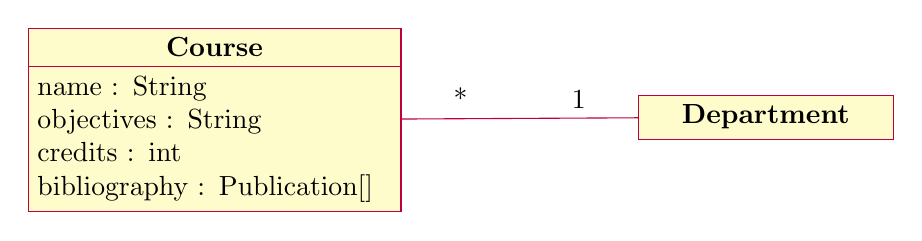
\begin{tikzpicture}

\begin{class}[text width=4.5cm]{Course}{0.5,0}
  \attribute{name : String} \attribute{objectives : String}
  \attribute{credits : int} \attribute{bibliography : Publication[]}
\end{class}

\begin{class}[text width=3cm]{Department}{7.5,-0.85}
\end{class}

\association{Department}{}{1}{Course}{}{*}

\end{tikzpicture}

\caption{Sample Domain Model in UML}
\label{fig:courseDomain}

\end{figure}

In this simplified domain model, a course belongs to a department, has
a name, its objectives, the credits granted upon completion, and the
recommended bibliography. The domain is deemed to be consistent only
if all attributes of course have a defined value, and each course must
have a department. Each department is responsible for managing its
courses, meaning that it is up to someone who works in the department
to start the process of creating new courses. The creation of a new
course should be executed transactionally, because other users of the
system should not be able to see a course in an inconsistent state.

There are several ways to implement this operation. I will now
describe two common scenarios for said implementation.

\subsubsection{Business Transaction in a single interaction}

A possible implementation of the course creation operation in a web
application is to have a single page in which the user provides all
the required information. Once the information is submitted, a new
\texttt{Course} is created, associated with the respective department,
and all its attributes are filled according to the information
submitted by the user. The new object is then stored in the database,
making it persistent and available for other users to view.

In this scenario, the transactional guarantees of the operation are
ensured by the underlying database (which is assumed to provide the
classic transactional semantics \cite{gray1981transaction}), because
the whole operation can be performed within the scope of a single
database transaction. An important consequence of implementing the
operation in a single database transaction is that the programmer can
manipulate all the domain objects involved directly. The order in
which the modifications to the objects are performed is irrelevant, as
long as the domain is consistent when the transaction is
committed. This is the semantics typically expected by a programmer of
such applications: There may be instants in which some domain objects
are in an inconsistent state (e.g. before defining the course's
bibliography), but this inconsistent state will never be seen by the
other users of the application. Those users will see the fully created
object only when the operation is committed.

\subsubsection{Business Transaction across multiple interactions}

The model described in the previous scenario may not be suited for
every situation. Imagine that instead of four attributes,
\texttt{Course} had 50 attributes. It would then be unfeasible to ask
the user to fill everything out in a single web page. So, one possible
solution would be to split the various attributes in multiple pages,
accounting for multiple user interactions. Let us now assume that the
creation of a course is made throughout three interactions. In the
first interaction, the user selects the course's name; in the second
interaction, the user introduces the objectives and credits; and in
the final interaction, the user selects the bibliography, thus
creating the course.

At first glance, it would seem quite easy for a programmer to change
the logic programmed in the first scenario to meet the new
requirements: The programmer would simply have to split the code
performed in a single request into three smaller parts, each to be
executed in one request. Yet, having three separate requests implies
having three different database transactions, breaking the atomicity
and isolation of the operation. After handling the first request, the
persisted domain would be in an inconsistent state (a course with no
attributes other than its name). The implementation of the business
logic must then take this issue into account, because the programmer
cannot write the updates directly on the domain. This scenario
represents what was defined as a Long-Lived Transaction, in which the
Business Operation has a larger lifetime that a single database
transaction (in this particular case, three database transactions).

\subsection{Why are they difficult to implement?}
\label{sec:difficult}

In this multiple interaction scenario, the programmer must take
special care when implementing the operation. There are several
possible choices:

\subsubsection{Keeping a database transaction open}

Given that atomicity and isolation are broken due to the fact that
each interaction with the user is done within its own database
transaction, we could think that the solution would be to keep the
database transaction open during the whole business transaction.

However, most modern Relational Database Management Systems (RDBMSs)
do not cope well with transactions that are open for arbitrarily large
periods of time, because a long lived database transaction may limit
concurrency, cause timeouts and deadlocks or starve the database's
connection pool. All these factors contribute to making this approach
highly undesirable, making the programmer seek alternative approaches.

\subsubsection{Parallel Representation of the domain}

In this approach, a series of objects similar to the domain objects
are created, and must be managed manually, kept in the user's session
context, outside the domain.

As the complexity of the domain and the number of objects manipulated
by the operation grows, it becomes harder for the programmer to manage
manually all of the data that must be kept. Ultimately, there is a
copy of the whole domain stored in the user's session, waiting for the
last transaction to update the domain with all the information entered
by the user.

This is the opposite of what would be desirable for the programmer:
She should be able to operate directly on the domain.

\subsubsection{Changing the domain model}

Now imagine that an additional requirement is added to the system: The
user may be allowed to log off in the middle of the process, and, upon
logging back in, continue the work where she left off. Additionally,
anyone else in the user's department should be able to pick up where
the original user left off. With these requirements, it becomes clear
that simply storing a copy of the domain in session-local storage is
not enough.

Web application containers already provide an application context,
which could potentially solve this issue. Unfortunately, there are no
real guarantees that the data stored in that context will be kept for
an arbitrarily large period of time (recall that our transaction may
span several days or weeks), meaning that the intermediate data must
be kept persistently, forcing the programmer to be concerned with this
issue.

A possible solution for this requirement is to change our domain
model, by adding a new attribute to the objects being modified (in
this case, \texttt{Course}). The \texttt{status} attribute
indicates whether the course is in a consistent state
(\texttt{Published}) or not (\texttt{Draft}). Adding this attribute
has a cost: Not only the domain becomes polluted with information that
is not relevant to the object being modeled, but this solution affects
other functional code across the application (e.g., course listings
must filter out courses that are still in the \texttt{Draft} status),
scattering the filtering code throughout the application.

\subsection{Objectives}

This Section shows that implementing Long Lived Transactions using
current transaction support systems is a rather difficult task that
promotes poor software engineering practices. As such, the work
presented in this dissertation aims at providing a solution that: (a)
Survives system restarts, ensuring that the intermediate data is
always available, (b) Provides the same correctness guarantees as
regular transactions, (c) Allows multiple users to collaborate
concurrently on the execution of a Long Lived Transaction, (d) Does
not impose an overhead on the execution of regular transactions and
(e) Shows performance results comparable to those of regular
transactions.


%% Related Work

\section{Related Work}
\label{chap:related}

In this section I describe the various areas in which an attempt to
solve the problem of Long Lived Transactions has been made, namely
Database Management Systems, Workflow Systems, and Object-Relational
Mapping Systems.

Also, due to its relevance regarding the solution described in section
4, I briefly present Software Transactional Memories (STM), Nested
Transactions, Persistent STMs, and how they cope with short lived
transactions.

\subsection{Transactions in Database Management Systems}
\label{sec:rdbms}

Transactions are an age-old notion in the database world. They
comprise a {\it Unit of Work} performed within a Database Management
System, and ensure that concurrent access to shared mutable data is
done in a consistent way.

By definition, a database transaction must provide the four ACID
properties:

\begin{itemize}

\item {\bf Atomicity} Requires that in a transaction, all database
  operations either {\it all} occur, or {\it none} occurs. This
  property guarantees that the transaction is indivisible and
  irreductible.

\item {\bf Consistency} Requires that every transaction will bring the
  database from one valid state to another (according to a series of
  consistency predicates defined for the database).

\item {\bf Isolation} Requires that individual record updates within a
  transaction are not visible outside of that transaction. When the
  transaction commits, all record updates are visible to the rest of
  the system.

\item {\bf Durability} Requires that once a transaction is committed,
  it will survive permanently. This means that once a transaction is
  committed, its effects on the data will be permanent.

\end{itemize}

\subsubsection{Isolation Levels}
\label{sec:isolation}

To better understand the desired isolation level of a Long-Lived
Transaction support system, an analysis of the most common isolation
levels is in order.

Attaining full isolation between transactions, while seemingly
necessary, can oftentimes be a burden to the DBMS, due to the required
overhead. Thus, isolation is, out of the four ACID properties, the one
most often relaxed. Isolation is typically implemented using Locks or
Multiversion Concurrency Control, which may result in a loss of
concurrency. To cope with that fact, several standard isolation levels
have been defined.

In the ANSI/ISO SQL standard\cite{melton1992ansi}, four isolation
levels have been defined (from most to least relaxed):

\begin{itemize}
\item {\bf Read Uncommitted} This is the lowest isolation level
  provided by any transaction support system. At this level {\it Dirty
    reads} may occur. A {\it Dirty read} is defined as a read
  operation that reads data updated by a live (not yet committed)
  transaction.
\item {\bf Read Committed} In this level, {\it Dirty reads} cannot
  happen (meaning they only read data written by already committed
  transactions). However, multiple reads to the same data location may
  read different values (from transactions that committed in between),
  even within a single transaction.
\item With {\bf Repeatable Read}, all reads within the same
  transaction read the snapshot established by the first read.
\item {\bf Serializable} is the {\it highest} isolation level defined
  in SQL. Serializability requires repeatable reads, as well as
  guaranteeing that {\it Phantom reads} do not occur. A {\it Phantom
    read} occurs when, in the course of a transaction, two identical
  queries (that act upon a range of values) return a different result
  collection. This can occur when running queries like ``SELECT * FROM
  users WHERE age BETWEEN 10 AND 30;''. If an interleaving transaction
  creates a new user with an age between 10 and 30 years, the second
  run of the query will show a result which contains the new user.
\end{itemize}

In \cite{papadimitriou1979serializability}, an extension to
Serializability is described: Strict Serializability. In addition to
the requirements for Serializability, Strict Serializability requires
that transaction histories are real-time ordered, meaning that all
transactions histories must be ordered in a way consistent with the
precedence order of the operations. In practice, this isolation level
is not implemented by DBMSs, due to its performance impact.

Another common isolation level (not described in SQL-92) is {\bf
  Snapshot Isolation}. In snapshot isolation, all reads made within a
transaction are guaranteed to see a consistent snapshot of the
database, and the transaction itself will only commit if no updates it
has made conflict with any concurrent updates since the
snapshot. Snapshot isolation arose from work on Multiversion
Concurrency Control, and thus did not make it into the lock-centered
mindset of the SQL-92 standard. This gap was heavily criticised in
\cite{berenson1995critique}.

\subsubsection{Concurrency Control}

Concurrency Control is the mechanism that ensures that ``Concurrent
execution should not cause application programs to malfunction''
\cite{reuter1993transaction}. This property was coined in 1993 as the
first law of Concurrency Control, by Jim Gray. In fact, concurrency
control mechanisms are what ensure that the ACID properties of
transactions are kept, in an environment with concurrent access to
shared mutable data. Research on the topic dates back to the 1970s
\cite{rosenkrantz1978system} and 1980s \cite{gray1981transaction}, and
is still a hot topic nowadays.

There are two main categories of Concurrency Control:

\begin{itemize}

\item {\bf Optimistic} Delaying integrity checking until the end of
  the transaction, without blocking any of its reads and writes.
  Optimistic concurrency control allows for greater concurrency,
  because concurrent operations can proceed without interfering with
  each other. On the other hand, given that integrity is only checked
  at the end of the transaction, conflicts are not detected until all
  the work is done and the transaction has to be restarted. It is
  typically implemented by Multiversion Concurrency Control and
  Timestamp Ordering mechanisms \cite{Bernstein1981}.

\item {\bf Pessimistic} Every data access in the transaction acquires
  a lock before proceeding. During the acquisition process, if an
  integrity violation is detected, the transaction is aborted, rolling
  back every write and releasing every lock held. Once the transaction
  is finished, it is marked as committed, and all the locks are
  released. The main method in this category is Two-Phase Locking
  \cite{Bernstein1981}.

\end{itemize}

Historically, pessimistic concurrency control has been the dominant
category, and even nowadays, most Relational Databases implement it.

Due to this fact, most of the work regarding Long-Lived Transaction
support in DBMSs is related with locking approaches. In fact, one of
the main reasons why databases do not cope well with long
transactions, is that the transaction holds a lock for each accessed
record. In lock-based DBMSs, the frequency of deadlock goes up with
the square of the concurrency level and the fourth power of the
transaction size \cite{gray1981transaction}. Thus, several strategies
have been devised to minimize the probability of deadlocks on
Long-Lived Transactions.

\subsubsection{Relaxation of Transactional Properties}

Given that holding the locks for the duration of the transaction was
not viable, the first proposed solution for this problem was to accept
a lower degree of consistency, by allowing transactions to release
their locks before commit.

In \cite{gray1981transaction}, the author proposed a model in which
only {\it active} transactions (the ones currently updating the
database) hold locks. {\it Sleeping} transactions (not currently
updating the database - also known as {\it User Think-Time}) do not
hold any locks. This means that the isolation property is broken, due
to the fact that other transactions will be able to see an uncommitted
value.

In \cite{salem1989altruistic}, the authors propose an extension to
Two-Phase locking, called {\it altruistic locking}. This extension
provides the concurrency control manager with a set of rules that
allow it to release locks early in the transaction. The altruistic
protocol takes advantage of the transaction's data access pattern. In
particular, it takes advantage of the knowledge that a transaction no
longer needs access to a data object that it has locked. Transactions
can then issue {\it release} operations, indicating that a certain
piece of data will no longer be accessed. Other transactions will be
allowed to access this data concurrently, while agreeing to abide by
certain restrictions that were put in place to ensure that all
transactions see a consistent database state.

\subsubsection{Transaction Logs}

Another problem with Long-Lived Transactions in DBMSs results from the
use of a Transaction Log, which contains a record of every operation
performed in the database, so that the DBMS can perform crash
recovery. The problem is that the size of that log is finite and, over
time, it fills up, thus forcing Long-Lived Transactions to abort, as
some of their log records will be overwritten by more recent
transactions.

In \cite{hagmann1991implementing}, the authors propose ``Log Record
Forwarding'', as a means to relocate log entries belonging to
Long-Lived Transactions, so that they will not be aborted for that
reason. In this proposal, active records in the log area are copied
(forwarded) to the end of the log, thus surviving another
log-reclaiming cycle.

\subsubsection{Sagas}
\label{sec:sagas}

Garcia-Molina and K. Salem proposed, in their 1987 paper
\cite{garcia1987sagas}, the notion of sagas. The basic idea of the
saga model is to allow a transaction to release resources prior to
committing. A Long-Lived Transaction is a saga if it can be seen as a
sequence of sub-transactions that can be interleaved in any way with
other transactions. Each sub-transaction in the saga guarantees that
the ACID properties on the database are preserved.

Partial executions of the saga are undesirable, so the DBMS is
responsible for guaranteeing that either all transactions in a saga
are successfully completed, or compensation actions are run to amend
the partial execution. Thus, each sub-transaction is associated with a
compensating transaction, which undoes the changes performed by the
original transaction. Note that this action does not necessarily
return the database to its original state, but instead acts upon the
{\it business state} of the application.

More formally, consider a saga $T$, consisting of sub-transactions
$T_1, T_2, \ldots, T_n$, and compensating actions $CT_1, CT_2, \ldots,
CT_n$. The system guarantees that either the sequence $T_1, T_2,
\ldots, T_n$ is executed (meaning the whole saga is executed), or
$T_1, T_2, \ldots, T_j,CT_j, \ldots, CT_2, CT_1$ for some $0 \le j \le
n$, will be executed (meaning that a failure occurred at $T_{j+1}$,
causing the previously executed sub-transactions to be compensated).

\subsubsection{Offline Concurrency Patterns}

Martin Fowler, in his book {\it Patterns of Enterprise Application
  Architecture} \cite{fowler2003patterns}, introduces a series of {\it
  Offline Concurrency Patterns}, as the building blocks for Long-Lived
Transaction support at the application level. In his patterns, Fowler
assumes that a Long-Lived Transaction is run as a series of
short-lived system transactions, whose transactional support is
provided by the underlying DBMS.

The patterns provide a workaround for the fact that the ACID
properties are broken when using several system transactions.

\begin{itemize}
\item {\bf Optimistic Offline Lock} This pattern solves the problem by
  validating that the changes about to be committed by one session (or
  business transaction) do not conflict with the changes of another
  session. This is achieved by, once the session is being committed,
  validating that the changes about to be committed are consistent,
  making sure that the value previously read by the current session
  was not changed by another session (i.e. obtaining an Optimistic
  Offline Lock).  The most common implementation of this pattern
  consists on associating a version number with the record in the
  system. When a record is loaded, the record's version is kept in the
  session, and that version is used when acquiring the Optimistic
  Offline Lock (by comparing the two versions). Once the lock is
  successfully acquired, the record's version is incremented, and the
  system transaction can be committed. If the lock cannot be acquired,
  a conflict is detected, the current system transaction is rolled
  back, and the business transaction must either abort or attempt to
  resolve the conflict and retry.

\item {\bf Pessimistic Offline Lock} This pattern prevents conflicts
  by avoiding them altogether. It forces a business transaction to
  acquire a lock in each record before using it, so once you begin the
  business transaction, you are mostly sure that it will complete
  without concurrency control issues. These locks however, are not
  database-level locks, but are instead high-level, typically managed
  by a lock manager in the application, and can have various
  granularities (which will have different impacts on system
  performance). In this pattern, whenever a business transaction
  wishes to access a record (for either read or write), it must
  acquire a lock with the lock manager, ensuring that a business
  transaction that wishes to write for that particular record is the
  only one doing so.
\end{itemize}

Typically {\bf Optimistic Offline Lock}s are used in an environment
where conflicts are expected to be low. If conflicts are likely, it is
not good user experience to report a conflict after the user finished
his work and is ready to commit. In that case, a {\bf Pessimistic
  Offline Lock} is in order, avoiding throwing away work, because
conflicts can be detected early in the transaction. Also, if the cost
of a conflict is too high, no matter its likelihood, this is the
appropriate pattern.

Although with the use of these patterns the development of Long-Lived
Transactions is facilitated, they require the programmer to pollute
the domain with the addition of code that should be at an
infrastructural level.

\subsection{Workflow Management Systems}

A Workflow Process is described as a sequence of connected steps (or
activities), with special emphasis on the flow paradigm, where each
step of the process follows the precedent, and ends just before the
next step can begin.

A Workflow Process typically may have a long duration, involve many
users (in fact, each step is typically executed by a different user),
and range across a variety of heterogeneous systems. Individual
activities range from computer programs and applications to human
activities such as meetings and decision making.

In this document I shall use an abstract model to describe Workflow
Processes, using the following concepts:
\begin{itemize}
\item {\bf Process} is a sequence of steps necessary to achieve a
  goal. A process consists of activities and data.
\item {\bf Activity} is each step within a process. Activities have a
  name, pre and post-conditions, and a series of constraints.
\item {\bf Control Flow} is the order in which activities are
  executed.
\item {\bf Data Flow} is the mapping between the inputs/outputs of the
  data required by the activities.
\item {\bf Conditions} specify the circumstances in which certain
  events will happen. {\it Transition Conditions} specify whether a
  certain activity may or may not become {\it startable}. {\it Start
    Conditions} specify when an activity is actually started, either
  by all its triggering events (AND) or by just one (OR). {\it Exit
    Conditions} specify whether an activity has finished successfully.
\end{itemize}
In this model, an activity with no incoming activities is considered a
{\it Start Activity}. A process is considered finished once all its
activities are terminated.

Over the years, many Workflow Modelling Languages have been devised,
and in fact, it is still a very active area of research. Examples of
such languages are YAWL \cite{van2005yawl}, AWGL
\cite{fahringer2005specification} and UEML \cite{vernadat2002ueml}, among
many others.

In \cite{sheth1993transactional}, the term {\it Transactional
  Workflow} was introduced, recognising the relevance of transactions
to workflows. Transactional Workflows provide functionality required
by each workflow process (such as task collaboration), which is
usually not available in typical DBMSs. This, however, does not imply
that workflows are similar to database transactions, nor that they
support all the ACID properties (namely concurrency control, backward
recovery, and data consistency).

Workflow Management Systems (WFMSs) are the systems that manage
user-defined Workflow processes for different types of jobs and
processes. It is the WFMS that provides the transactional properties
to the transactional workflow. These include transaction management
techniques such as logging, compensation, etc.

Given that their support for recovery and failure handling is lacking,
unlike regular transaction systems, they typically provide the means
for the user to determine the actions necessary to recover from
failure and consistency issues.

\subsubsection{Implementing Transactional Workflows}

In \cite{dayal1990organizing}, a workflow is seen as a {\it
  Long-Running Activity}, and is modeled as a set of execution units
that may consist recursively of other activities, or top-level
transactions. Control and data flow is specified either statically in
the activity's {\it script}, or dynamically using
Event-Condition-Action (ECA) rules. This model contemplates
compensation, execution unit communication, activity status queries
and exception handling.

In \cite{weikum1993extending}, the author suggests that semantic
transaction concepts be merged with workflow concepts to promote
consistent and reliable workflow systems. The author defines a
transactional workflow to be a control sphere that binds these
transactions, using dependencies to enforce as much behavioral
consistency as possible.

For a more comprehensive review on the topic, refer to
\cite{worah1997transactions}.

\subsubsection{Sagas}

The concept of Sagas was previously presented in
Section~\ref{sec:sagas}. In this section, I show how sagas can be
implemented on top of Workflow Management Systems.

All the sub-transactions of the saga are grouped into a block (Forward
Block). The control flow within the block represents that of the saga,
with each sub-transaction represented as an activity. Every activity
has an incoming transition condition, which is that the previous
activity has finished successfully (i.e. the corresponding transaction
has committed).

If a transaction aborts, the corresponding outgoing condition will
evaluate to false, and no other activity in the block will
execute. When execution of the block terminates, its data container
will contain a list of the status of each activity. In this case,
control is passed to a second block (Compensation Block), containing
the compensating activities in reverse order.

When the compensation block is executed, all the conditions that
correspond to activities that executed in the Forward Block are
activated, causing the compensating activities to be executed in
order.

\subsubsection{Implementing Long-Lived Transactions using WFMSs}

As described in the previous sections, several attempts have been made
to implement Advanced Transaction Models on top of Workflow Systems,
as a means of supporting Long-Lived Transactions.

Several other methods have been proposed in the literature (e.g.,
\cite{alonso1996advanced, 798492}). However, such implementations are
not suitable for the requirements defined in Section~\ref{sec:what},
due to the fact that most WFMSs do not provide full ACID properties.

\subsection{Object-Relational Mapping}
\label{sec:orm}

Due to the increase in popularity of object-oriented programming, a
large number of Object-Relational Mapping (ORM) tools have arisen over
the past few years \cite{orm}. These tools range from simple data
access layer abstractions (which simply abstract the necessary
instructions to perform the desired operation), to fully fledged
tools that handle every aspect of the Object-Relational Mapping,
making the underlying database completely transparent to the
programmer.

Object-Relational Mapping tools are available for a great number of
languages. For Java, there are many competing persistence standards,
including: Java Persistence
API\footnote{\texttt{http://jcp.org/en/jsr/detail?id=317}} (JPA), Java
Data
Objects\footnote{\texttt{http://www.jcp.org/en/jsr/detail?id=243}}
(JDO), Spring
Data\footnote{\texttt{http://projects.spring.io/spring-data/}}, among
others. Both specifications allow a programmer to create domain
entities by decorating Plain Old Java Objects (POJOs) with
annotations, making the persistence layer transparent to the
programmer. Whereas JDO provides a larger number of features than JPA,
the latter has seen greater adoption by the community, both in terms
of usage and support. The most well-known implementations of the JPA
are Hibernate (\texttt{http://www.hibernate.org}), OpenJPA
(\texttt{http://openjpa.apache.org}) and EclipseLink
(\texttt{http://www.eclipse.org/eclipselink/}).

To provide transactional support for domain objects, ORMs typically
delegate transaction management to the underlying Database (which is
assumed to provide full ACID support). In fact, as of this writing,
all the examples shown above operate this way. Thus, Long-Lived
Transaction support in ORM tools is largely dependent on the
underlying DBMS, presenting the same challenges as described in
Section~\ref{sec:rdbms}.

Given the popularity of Java, I will now consider the JPA, and one of
its most popular implementations, Hibernate, to understand how they
cope with Long Lived Transactions. Note that despite the concreteness
of the examples presented, their concepts are generic enough to be
applied to any other ORM tool.

\subsubsection{JPA Optimistic Concurrency Control}

The specification of the Java Persistence API assumes the use of
optimistic concurrency control (or optimistic locking). In this
context, optimistic locking is used to prevent the database from
holding on to critical resources, potentially causing high degrees of
contention.  This is achieved by operating directly on the domain
objects (in memory), delaying the propagation of the changes to the
database as much as possible.

As part of the JPA, there is the concept of Version field. This field
allows {\it disconnected operation}, meaning that the reads/writes
from the database are deferred until a checkpoint or the end of
transaction. When using this optimistic approach, all the versions of
the objects used in the transaction are checked against the version
present in the database, thus ensuring that no dirty reads will occur.

\subsubsection{Hibernate Long Conversations}

Hibernate supports the concept of {\it Long Conversations} by allowing
a session\footnote{A Hibernate session implements the Unit of Work
  design pattern \cite{fowler2003patterns}.} to remain open as long as
the user interaction lasts, potentially executing multiple database
transactions. However, the programmer is responsible for ensuring the
atomicity and isolation of the business transaction, by following a
very strict pattern: All transactions but the last must only read
data, and, thus only the last database transaction can update
data. Hibernate assists the programmer in verifying that the data read
across the multiple transactions is consistent, using an object
versioning mechanism. However, this verification only works if all the
data required for the application is read within the first database
transaction.

This support is not good enough for several reasons:

\begin{itemize}
\item It imposes a pattern that may not be suited for many
  applications.
\item All the state of the transaction is kept in memory, which may
  cause the application to run out of memory in very large
  transactions.
\item The session is not kept persistent. If the application server
  restarts in the middle of the transaction, all data related to the
  ongoing Long Conversation is lost.
\item Despite the versioning support, the business transaction may
  still suffer from inconsistent reads, as it spans multiple isolated
  database transactions. Suppose that in a database transaction (T2)
  other than the first one (T1), the application reads an object for
  the first time. If the object was concurrently modified by yet
  another transaction (T3) that occurred between T1 and T2, T2 would
  see the value written by T3, which would not be consistent. As such,
  these transactions are not {\it Serializable} (See Section \ref{sec:isolation}).
\end{itemize}

All of these reasons violate the desired properties described in
\ref{sec:difficult}, making this system undesirable.

\subsection{Software Transactional Memories}
\label{sec:stm}

Given that the solution I propose in Section \ref{sec:arch} is built
upon a Software Transactional Memory (STM), I provide here a brief
introduction to the topic.

The original idea behind Transactional Memories (TM)
\cite{herlihy1993transactional} is to provide efficient lock-free data
structures for highly concurrent systems using hardware. Its main goal
was to free programmers from using locks and monitors to manage
concurrent accesses to shared data. Managing lock granularity and
composability is a cumbersome and error-prone task, and may lead to
unwanted situations such as deadlocks. Over the years, the original
concept of Hardware Transactional Memories has evolved, giving birth
to Software Transactional Memories \cite{shavit1997software}.

Software Transactional Memories bring into the realm of programming
languages, the age-old notion of transactions, well-known in the area
of DBMSs. However, unlike those, STMs are not concerned with the
Durability property of the ACID model, and thus, many STM
implementations have little in common with their database
counterparts.

There have been several recent proposals for STM implementations, such
as those described in \cite{cachopo2006versioned, herlihy2003software,
  marathe2005adaptive, dice2006transactional, riegel2006lazy,
  marathe2006lowering}.

STMs use transactions to isolate memory operations in atomic Units of
Work. A transaction typically contains a Read Set and a Write Set,
which are used to register its read and write operations,
respectively. The STM provides a series of mutable memory locations
that can be read from or written to. In many STMs, it is up to the
programmer to confine all of the application's mutable state to these
memory locations, whereas some STMs provide fully transactional
memory. It is the responsibility of the STM to guarantee that
concurrent accesses to such memory locations are correct according to
the specified correctness criteria.

\subsubsection{Correctness Criteria}
\label{sec:opacity}

In Section~\ref{sec:isolation}, I presented the typical isolation
levels (or correctness criteria) that can be found in DBMS. In
\cite{guerraoui2008correctness}, the author claims that the {\it
  traditional} correctness criteria are unfit for TM implementations,
and proposes the {\it opacity} criterion. Opacity is described as a
safety property that ensures that ``[...] (1) all operations performed
by every {\it committed} transaction appear as if they happened at
some single, indivisible point during the transaction lifetime, (2) no
operation performed by any {\it aborted} transaction is ever visible
to other transactions (including live ones), and (3) every transaction
always observes a {\it consistent} state of the system.'', meaning
that unlike Serializability, even {\it non-committed} transactions are
prevented from accessing inconsistent states. This correctness
criteria is ensured by many TM systems.

\subsubsection{Nested Transactions}

The best practices in software development encourage programmers to
modularize their applications and have them abide by well-defined
interfaces. Lock-based approaches do not cope well with this
principle, because the programmer must be aware of module's internal
locking conventions. Transactions, on the other hand, do not have this
limitation, allowing for better composability.

In the transaction paradigm, it would then be common for application
code to make a call to a library that uses transactions to protect its
shared internal state. In this scenario, the transaction created by
the library would be {\it nested} in the outer (application-owned)
transaction. Nested Transactions are an extension to the basic
transaction structure, supporting multiple levels of transactions:
Transactions that may contain other sub-transactions, forming a
transaction tree. Nested Transactions have long been used in the
database world, and many of its concepts have been adapted to
transactional memories.

Consider the kind of monolithic transactions commonly found in
enterprise applications. In such transactions, the volume of work that
must be done if the transaction needs to be rolled-back is
increased. Using nested transactions, smaller portions of the work can
be done in isolation, each within a nested transaction. If one of
those portions fails, only that portion needs to be rolled-back, and
an attempt can be made to compensate for that failure. Similarly,
clients of opaque libraries may suffer performance hits if the
transaction fails because of the work performed in said libraries.

In \cite{moss2006nested}, Moss and Hosking defined two types of
nesting: Closed and Open.

\subsubsection{Closed Nesting}

A transaction is either {\it top-level}, which is similar to a
non-nested transaction, or is nested within a {\it parent}
transaction. In this model, only transactions with no current children
can access data. Transactions accumulate Read and Write sets, which
will determine the outcome of the transaction. When a transaction
reads a value, it sees either the value in its own read or write set,
or the value seen by its parent (a top-level transaction sees the
latest value).

When a nested transaction commits, its read and write sets are merged
with the ones of its parent. It is only when the top-level transaction
commits that its writes become permanent. If the nested transaction
aborts, its read and write sets are discarded.

\subsubsection{Open Nesting}

Open Nested Transactions relax the isolation requirements by making
the results of committed sub-transactions visible to other
concurrently running transactions. When a sub-transaction commits,
instead of merging the write set with its parent's, the writes are
committed at the top-level. This way, a higher degree of concurrency
is achieved, because resources may be released earlier and conflict
detection can be applied at a higher level. It is up to the
implementations to provide the mechanisms to handle recording of
necessary compensating actions in case an ancestor transaction aborts.

\subsubsection{Nested and Long-Lived Transactions}

Nested Transactions present many similarities with Long-Lived
Transactions. In both cases there is a top-level transaction, which
can be divided in several smaller steps. Open nesting uses the same
basic principle as the techniques described in previous sections,
based on the relaxation of transactional properties, and compensating
actions. Closed Nesting is similar to the desired properties presented
in Section~\ref{sec:what}.

\subsection{Persistent STMs}
\label{sec:pstm}

Over the years, Enterprise Application architecture has evolved at a
very fast pace. However, one aspect has remained constant: They still
rely on a relational database to handle both data persistence and
transactional support. In \cite{fernandes2011strict}, the authors
argue that such design, while once justified by hardware limitations,
is no longer suited for today modern applications.

A new architecture was proposed, using a Software Transactional Memory
for transaction support at the application server tier, shifting the
responsibility from the DBMS to the application server. The database
still plays an important role in this architecture, due to the fact
that the STM must be extended to support persistence (PSTMs).

By shifting the responsibility for transaction handling to the STM,
enterprise applications can benefit from the many advancements in the
STM area, such as multi-core machine scaling, stronger correctness
guarantees and nonblocking progress conditions such as lock freedom
\cite{fernandes2011lock}.

Using a PSTM, enterprise application developers no longer have to
trade correctness for performance. Modern PSTM implementations allow
for Strict Serializability, while providing better performance than
regular DBMSs, yielding a throughput increase of up to 23 times
\cite{fernandes2011strict}.

Another advantage of PSTMs is that, like in STMs, the programmer
benefits from a much simpler and transparent programming model,
allowing for much cleaner and maintainable code, better composability
by using lock-free data structures, making the process of translating
business requirements to code much simpler and bug-free.

In this project, I aim at extending the PSTM model, by adding the
necessary building blocks to support Long-Lived Transactions
(described in Section~\ref{sec:arch}).

\subsection{Why those solutions are unfit}

Among all the solutions presented above, one common aspect stands out:
They all require the programmer to deal with Long-Lived Transactions
at the application level, which goes against my claim that support
should be transparent, and at an infrastructural level.

Some of the presented solutions are based on relaxation of
transactional properties, such as allowing breaches in
isolation. Long-Lived Transactions should run with the same
transactional properties as regular transactions, and thus, relaxation
is not acceptable.

Despite the similarities between Workflow Processes and Long-Lived
Transactions, WFMSs are not suited for our requirements. Typical WFMSs
are not concerned with the ACID properties of transactions, and rely
heavily on high-level compensatory actions for data consistency.

The solution proposed in Section~\ref{sec:orm} (Hibernate) imposes a
very strict programming model, which may not be adequate for some
applications, and does not guarantee that Long-Lived Transactions will
have the same transactional properties as regular transactions.

None of the proposed solutions fit the requirements specified in
Section 2, and thus, a new approach is needed.

%% FF

\section{Fenix Framework}
\label{chap:ff}

This chapter describes in detail the major components of the Fenix
Framework, which is the Framework used to implement the solution
proposed throughout this document. Section \ref{sec:dml} describes the
Domain Modelling Language, used to describe the application's domain
model. Section \ref{sec:ff-arch} describes the high-level architecture
of the Framework, briefly describing its major components and their
interaction. Section \ref{sec:codeGen} describes the process of Code
Generation. Section \ref{sec:jvstm} presents the Java Versioned STM
(JVSTM), and its integration with the Fenix Framework. The information
presented in this chapter is critical to understanding the proposed
solution, as well as its challenges.

\subsection{Domain Modelling Language}
\label{sec:dml}

The Fenix Framework is aimed at entreprise-class applications with a
rich domain model in an object-oriented paradigm. Such applications
typically consist of class hierarchies representing entities with
relationships among them, forming an interconnected graph. 

The Domain Modelling Language (DML) is a Domain-Specific Language
designed to represent such domain models, separating the domain's
structure from its behaviour. The DML is designed with modularity as a
core concern, allowing for incremental and modular domain definition.

In a DML file, programmers write their domain definition in a
Java-like language. A class definition consists of the class name, the
entity slots (either primitive or value types), and the super
class. Listing \ref{list:class-example} shows how the \texttt{Course}
and \texttt{Department} classes from Figure \ref{fig:courseDomain}
could be described in the DML. Note that as arrays are not natively
supported, a Value Type must be created, describing an array of
publications. Value Types are described in more detail below.

\begin{lstlisting}[caption={DML for the \texttt{Course} and 
  \texttt{Department} classes},
  label={list:class-example}, float]
class Course {
  String name;
  String objectives;
  int credits;
  PublicationList bibliography;
}

class Department {
  String name;
}
\end{lstlisting}

Relations in DML are named, first-class citizens that represent
relationships between two classes. Relations are always bi-directional,
meaning that updating one side of the relation will automatically
update the other side. Relations can be concealed in one of the sides
(meaning that it will not be possible to access it), however their
state is still kept.

It is possible to define {\it one-to-one}, {\it one-to-many} and {\it
  many-to-many relationships}, and it is possible to define boundaries
on the multiplicity of each relation (for example, a
\texttt{Department} can have between 0 and 30 \texttt{Courses}). Any
violation to these constraints would put the relation in an
inconsistent state and is discarded.

To-many relations in the Fenix Framework have Set semantics, meaning
that an object can only be present in a relation once. Also, there are
no ordering guarantees when accessing the relation.

Consider the relation between the \texttt{Course} and
\texttt{Department} classes shown Figure~\ref{fig:courseDomain}. The
relation would be given a name that describes the relationship between
the two classes, as well as names to describe the role each class
takes in the relation. The multiplicity is defined for each of the
roles, in this case, one \texttt{Department} has zero or more
\texttt{Courses}, and one \texttt{Course} has between one and one
(exactly one) \texttt{Department}.


From the domain definition, the Fenix Framework generates Java getters
and setters for the properties and relations. For each class described
in the DML, two Java classes are created: the domain class, in which
programmers can include business logic, and a \texttt{Base} class
(which the domain class extends) containing generated methods to
access the persistent entities of the object.

\subsubsection{Value Types}

In the DML there is a distinction between entities and value
objects. Whereas an entity is transactional and persistent, a value
object is immutable and not persistent. Value objects are used as the
values for slots of DML classes, and must be of well-known types,
known as Value Types.

A value type contains information regarding the Java Type (such as
\texttt{java.math.BigDecimal}), an alias (such as
\texttt{BigDecimal}), and information regarding how the object will be
externalised/internalized.

There are two categories of Value Types: Builtin (Java Primitives and
their wrappers, Enums, JodaTime types, JsonElement, and byte arrays)
and user-defined. User-defined types allow the programmer to use any
type they wish as a slot, provided the type is immutable (explanation
as to why is provided ahead) and can be expressed in terms of other
Value Types.

The Framework knows how to handle Builtin Value Types (i.e. how to
store/retrieve from persistent support). User-defined, on the other
hand, require that the programmer specify how the type is
externalised/internalized. The externalised type must be either a
Builtin Value Type, or a used-defined type that ultimately is
externalised to a builtin type.

\subsubsection{JSON}
\label{sec:json}

JSON (JavaScript Object Notation) is described as being ``[...] a
lightweight data-interchange format''. JSON is quickly becoming the
de-facto standard to interchange data across heterogeneous systems,
replacing XML in many cases.

As such, in the context of this work, the Framework was extended to
provide native JSON support (by allowing it as a Builtin Value Type),
using Google's GSON\footnote{\url{http://code.google.com/p/google-gson/}}.
Using JSON allows the programmer to define arbitrarily complex Value
Types with little effort, as well as simplifying externalisation code.

The Framework also provides support to transform any Value Type
to/from JSON, meaning that a JsonElement slot is enough to keep any
value the Fenix Framework is able to handle. As shall be presented in
Chapter~\ref{chap:solution}, this proves to be a crucial feature.

\subsection{Architecture}
\label{sec:ff-arch}

The first versions of the Fenix Framework (as presented in
\cite{fernandes2011strict}) had a rather monolithic
architecture. Transactional support was provided by the JVSTM (see
Section \ref{sec:jvstm}), and persistence was implemented on top of
MySQL, leaving the programmer with no other choice of technology.

With the second major version of the Framework (released earlier this
year), a great architectural shift has occurred. There is now a clear
separation between the Framework's public API and the
transactional/persistence backends, allowing for a ``write once, run
everywhere'' paradigm. The programmer simply writes his application
against a public API and is able to run it on multiple backends.

This way, not only are applications portable across several
technologies (MySQL, Neo4j, Hibernate, etc), but also testing support is
greatly enhanced, as there is no need to mock the persistence API, as
tests can be run using an in-memory backend.

Figure~\ref{fig:ff-arch} shows the major modules that constitute the Fenix
Framework.

\begin{figure}
\centering
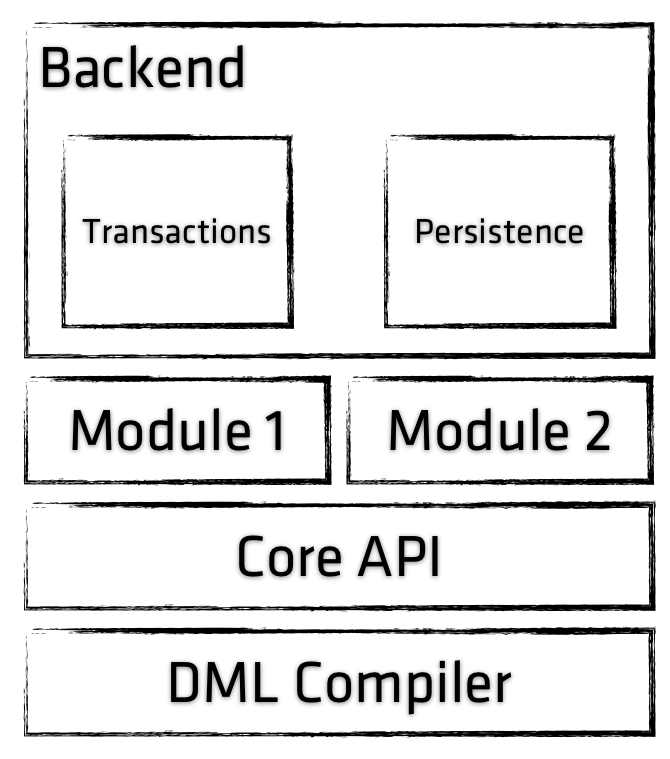
\includegraphics[width=0.8\linewidth]{ff-arch}
\caption{Fenix Framework's Layered Architecture}
\label{fig:ff-arch}
\end{figure}

The DML Compiler module contains the parser responsible for reading
DML files and creating an in-memory description of the Domain Model,
as well as all the necessary classes to represent it. It also contains
the base \texttt{DomainObject} interface, which all objects of the Domain
Model implement. Also present in this module are the base Code
Generators used to create the Base classes for all domain
objects.

The core of the Framework is in the \texttt{Core API} module. Transaction
management APIs, configuration, entry points, backend interfaces, are
all defined in this module.

Many backend-independent modules are provided with the Fenix Framework
bundle. These include persistent Abstract Data Types (B+Trees, Linked
Lists, etc), support for Consistency
Predicates \cite{JoaoCoutinhoNeves2011}, statistics collection tools,
indexing and transaction introspection. These modules are used
internally by the various backends, but can (and in most cases should)
also be used by the programmers.

Backends provide the concrete implementations of transactional and
persistence support, and are required for applications to work.

\subsubsection{Public API}

One of the major advantages of the Fenix Framework is that
applications built on top of it are independent of the underlying
persistence and transactional backend. However, to guarantee this
property, the modules that form such applications must be compiled
against the Public API of the Framework.

The public API is split in two major components:

\begin{itemize}
\item {\bf DML Compiler} Allows applications to have runtime access to
  the structure of the domain and allows registering relation
  listeners that will be invoked each time a relation is
  modified. This module also defines the API that is generated based
  on the DML, which must be supported by all backends.

\item {\bf Core API} Provides the entry point for the domain's object
graph through the \texttt{DomainRoot} class, the mechanism to retrieve a
Domain Object from its unique identifier, transaction APIs that can be
used to either mark a piece of code as transactional (@Atomic
annotation) or to manually manage the lifecycle of transactions, and
utilities to configure the Framework.
\end{itemize}

With this separation, the classpath of the application modules is not
polluted with implementation details, allowing for a faster
development and test cycle.

\subsubsection{Backends}

Backends are a crucial part of the Fenix Framework. They provide
concrete implementations of the transactional and persistence
support. Application modules should not depend directly on the
backends, as their API is private and as such subject to change even
among minor versions, and having a dependency on a specific backend
means that portability must be sacrificed.

The fact that backends have a clear separation from the Public API
allows for a much faster evolution of the backend's
implementation. Major internal changes can be done without affecting
the end-users directly, even in a revision release, whereas changes to
the public API require either a major or minor release.

\subsection{Code Generation}
\label{sec:codeGen}

As previously described, access to persistent fields of domain objects
is done using generated methods in Base classes.

Code generation is closely tied to the specific backends, as it is
typically used to support the process of persisting an object to a
database. An example of an operation performed in generated code is
binding a \texttt{PreparedStatement} with the values of the object's
slots, or externalizing the object to JSON.

There are two major components in code generation:

\begin{itemize}

\item The default code generator, from which every other generator
  inherits, defines the public generated API for domain classes. Its
  major use-case is to compile backend agnostic application modules
  that only need base classes because of their API (modules aren't
  bundled with base classes, those are generated on-demand on
  depending modules or applications).

\item Backend-provided code generators. These generators extend the
  base ones, thus providing the same API, using backend-specific
  artifacts to fullfil the API. Backends can also use code generators
  to optimise runtime performance, by injecting in generated code
  values that otherwise would have to be computed at runtime.
\end{itemize}

Whereas this Code Generation architecture allows for great
optimizations (it allows backends to perform complex operations
without resorting to reflection), it comes with a tradeoff: Forcing
the domain classes to inherit from Base classes hinders the
readability of the code (as the user is required to either check the
DML or the base class to find out the super class), makes it
impossible to invoke constructors of the super class (as the Base
class only generates the no-arg constructor), does not allow the
programmer to choose the visibility of the generated methods (as they
are always generated public) among other issues.

The Code Generation step also provides a mechanism to transfer
compile-time information to the runtime. Information such as the App
Name (which is used at runtime to generate the graph of DML
dependencies), the name of the Backend used to compile the final
application (to allow for automatic initialization), as well as pass
user-defined parameters to runtime.

\subsection{JVSTM}
\label{sec:jvstm}

The Java Versioned Software Transactional Memory (JVSTM)
\cite{cachopo2006versioned} is a pure-Java implementation of a
Software Transactional Memory (see Section~\ref{sec:stm}).

The JVSTM uses the concept of Versioned Boxes (VBoxes) to make a
memory location transactional, keeping the history of values for that
position, one for each version of the box. Reads and writes to VBoxes
are tracked by the JVSTM in a per-transaction basis.

Each transaction begins at a given moment, acquiring the version
number at that moment. The version number is used during the
transaction to ensure that all reads get the correct value at the time
of the transaction's start, thus providing Opacity guarantees
\cite{guerraoui2008correctness}. This allows for conflict-free
read-only transactions, as concurrent transactions writing to the read
boxes will write a new version instead of overwriting its previous
value.

\subsubsection{Integration}

The JVSTM is integrated with the Fenix Framework, as one of the
multiple available backends. This document focuses on the backend
named \texttt{jvstm-common}. This backend uses the JVSTM for the
transactional support, while abstracting the persistence
details. Despite being meant to be extended, \texttt{jvstm-common}
provides an in-memory implementation of the persistence API.

The implementation of the solution proposed in
Chapter~\ref{chap:solution} rests on top of this abstract backend,
meaning that it will work on top of any persistent support, as long as
the JVSTM is used.

In this backend, Base classes use VBoxes to store the value objects
transactionally, thus taking advantage of the JVSTM. The generated
getters and setters are backed by \texttt{VBox.get()} and
\texttt{VBox.set()}, and can be invoked only from within a
transaction.

\subsubsection{VBoxes}

A plain JVSTM VBox is simply a wrapper to a Linked-List of pairs
[Version, Value], containing the history of values for that box.

A Fenix Framework VBox however, also contains a back-pointer to its
owner, as well as the name of the slot it represents. This allows for
the persistence support to know where to store the value of the Box.

Those specialised VBoxes can have their previous values
Garbage-Collected and reloaded from persistent support on-demand.

\subsubsection{VBoxes for slots}

There are two layouts for Domain Object's slots: {\it (1)} Using one
VBox to keep the entire state of the object (One-Box), and {\it (2)}
Using one VBox per slot (Multi-Box).

The first layout suffers from a higher number of conflicts, as reading
one slot will conflict with writing another slot on the same object
(as they are mapped to the same VBox), however the memory usage is
much lower, as each VBox has a cost for its underlying data
structures. This aspect is critical in applications with a dense
domain model, with many objects and many slots.

Smaller applications can use the Multi-Box layout to greatly reduce
conflicts. In this layout, each domain slot is given its own VBox.

In both layouts, a specialised VBox called \texttt{PrimitiveBox} is
used to store either the object's state or the slot's value. There is
no added behaviour or data in a PrimitiveBox, however persistence
support uses this information to determine whether to reload a box
containing the state (or part of it) of an object or a box for a relation.

\subsubsection{VBoxes for relations}

In the One-Box layout, to-one relations are kept inside the object's
state, and as such require no special handling. 

On the other hand, for a Multi-Box layout, the reference to the
related object is kept in a \texttt{ReferenceBox}. Just like a
\texttt{PrimitiveBox}, it contains no extra behaviour or data, and
serves only as a marker for persistence support to know it has to load
an object reference.

To-many relations however, are handled in a very different manner. The
preferred approach is to use a B+Tree \cite{elmasri2009fundamentals}
to store the objects on the to-many side of the relation. For each
to-many relation, a {\it ReferenceBox} is generated, containing a
reference to the domain object representing the B+Tree.

The Fenix Framework provides an implementation of persistent B+Trees
that does not use to-many relations (by design, so it can be used to
implement them). In this implementation, each node of the tree is a
domain object containing only a reference to its parent and its
sibling. Inner nodes use an immutable TreeMap wrapper to keep indexed
references to the nodes they point to. Leaf nodes follow the same
strategy, keeping the mapping between keys and the objects they point
to (in reality they can be used to point at anything, however for this
document we are only interested in B+Trees containing domain objects).

As a B+Tree is generically a key-value map, its usage can be twofold:
provide a simple way to implement to-many relations and provide
support for relations indexed by a slot of the related
object. Consider the previously presented {\it Course} example. In
this model, one Course has many Students. As such, there is a B+Tree
slot in the Course Base class, which contain the references to all the
students enrolled in that particular course.

In the usual scenario, the B+Tree contains a mapping between OIDs and
the respective target object (which is rather useless, as the Fenix
Framework provides a lightweight API to read an object by its OID).
Now consider a scenario where the set of students must be indexed by
student name. The B+Tree will now contain a mapping between the
student's name and the target student, allowing for indexed lookups of
students by name.

%% Solution

\section{Solution}
\label{chap:solution}

With a proper understanding of the Fenix Framework, this chapter
describes the solution proposed to simplify the development of Long
Lived Transactions. Section~\ref{sec:arch} describes the architecture
of the proposed solution, with the rationales for each design
decision. Section~\ref{sec:impl} describes how the proposed
architecture was implemented on top of the Fenix Framework using the
JVSTM. Finally, Section~\ref{sec:validation} shows that both the
architecture and implementation fullfil all the requirements, and
attempts to measure the effort required to use the implementation.

\subsection{Architecture}
\label{sec:arch}

The main goal of this work is to relieve programmers of the burden of
dealing with Long Lived Transactions, making the effort needed to
program an LLT similar to the effort of programming a regular
transaction.

So, what does the single interaction scenario has that makes it so
easy to program? It has a single transactional context that spans the
whole operation (provided by the STM transaction). In the multiple
interaction scenario the system transaction was shorter than the
business transaction, so in each step the context was lost.

Looking at the information that is kept during the lifespan of a
regular transaction, we can identify three major pieces:

\begin{itemize}
\item The version in which the transaction is running. This version
  number corresponds to the logical point in time at which the
  transaction started.
\item A list of all the items written throughout the transaction (and
  the respective written values). This is the critical piece, as it
  contains the updated data that will be written to the global state
  of the application on transaction's commit.
\item A list of all elements read throughout the transaction. This
  piece of information is critical to ensure the correctness of the
  operation, as the outcome of the transaction may depend on the
  values of all the read data.
\end{itemize}

These pieces are crucial to ensure the correct operation of an
STM-based transactional system. STM libraries provide them for regular
(short-lived) transactions. The solution presented below aims to
provide them for Long Lived Transactions, using the short-lived
transactions as its building blocks.

Short lived transactions keep all the necessary information in
transient transaction-local storage (typically in memory), until the
time they commit, merging the write set with the global state of the
application. With Long Lived Transactions, merging this write set in
each step is not possible.

Recall the Course creation example. Consider that in the first step a
Course is created with only a name and the department it is associated
to. Merging the Write Set for this step with the global state would
leave the system in an inconsistent state in which the departement is
associated to an unfinished course, as this transitory state would be
visible to the outside world.

There needs to be a way to persistently store the Write Set of each
step, outside the global state of the application so that the changes
are not visible to the outside world. Only upon committing the Long
Lived Transaction these changes would be merged to the global state,
meaning that the writes performed by each step are effectively delayed
until the end of the transaction. Note that for correctness purposes,
the Read Set of the transaction must also be collected, so that at
commit time both Read Set and Write Set can be replicated, taking
advantage of the already existing JVSTM support.

As the main feature of the Fenix Framework is providing mechanisms to
manipulate transactionally and to persist Domain Objects, perhaps it
would be a good approach to use regular Domain Objects to store the
required information.

\subsubsection{Data Structures}

\begin{figure}
\centering
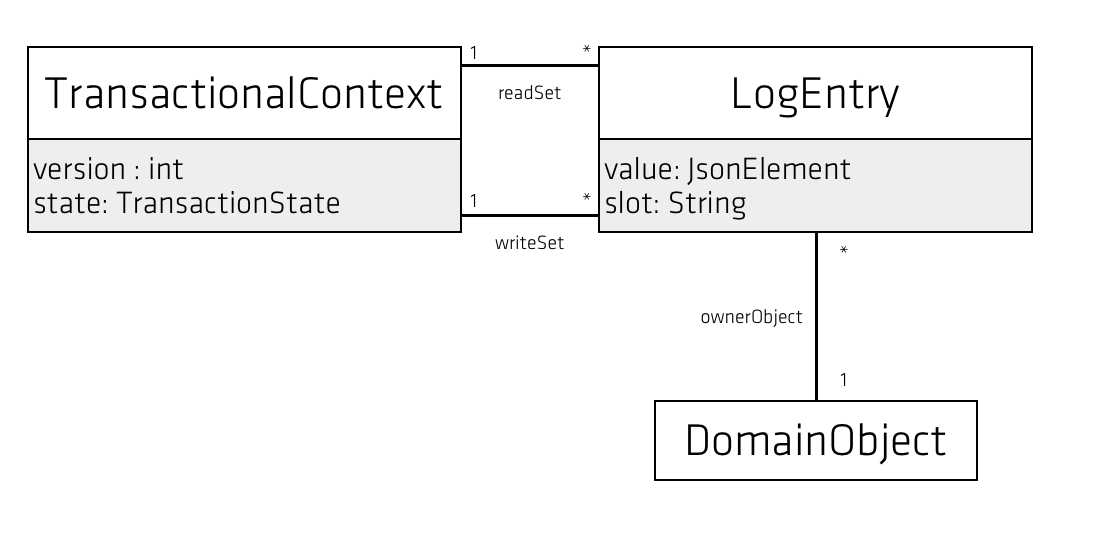
\includegraphics[width=0.5\linewidth]{tx-context}
\caption{Transactional Context's Domain Model}
\label{fig:transactionalContext}
\end{figure}

Consider the domain model presented in
Figure~\ref{fig:transactionalContext} that represents the reification
of the necessary data necessary for a transaction. A
\texttt{TransactionalContext} is the centerpiece of the domain, it
represents a Long Lived Transaction, holding together the entire state
of the transaction. By keeping the state of the LLT in regular domain
objects, we are ensuring that it is stored persistently (or at least
as persistent as the rest of the application) as well as
transactionally safe. Updates to the context are performed using a
regular transaction, allowing for multiple users to concurrently run
LLT steps (which will simply perform reads and writes to the context).

In this model, the \texttt{TransactionalContext} keeps the state of
the transaction (whether it is started, committed, aborted or in
conflict) and the version marker (corresponding to the ``current''
version when the first step of the transaction executed).

A \texttt{TransactionalContext} has two associated sets of
\texttt{LogEntries}, one for the Read Set and one for the Write Set. A
\texttt{LogEntry} represents one read or written slot throughout the
transaction, by keeping a reference to the object, slot name, as well
as the value that was written (note that the value is only kept if the
LogEntry belongs to the Write Set).

\subsubsection{Transaction Isolation}

Having the necessary data structures laid out is crucial for a proper
implementation of Long Lived Transactions, but it is just the
beginning. Whereas these structures are agnostic to the specific
backend, the backend must be able to recognise when a transaction is
executing within the context of a Long Lived Transaction, so that
reads and writes are isolated from the global state of the application
(otherwise the whole world could see the intermediate values).

In the Fenix Framework, transactions are bound to a specific thread,
allowing for multi-threaded applications to execute multiple
concurrent transactions, each one in its own thread. As such, to run a
transaction in the context of a Long Lived Transaction, one must first
bind the context to the current thread. This way, when beginning a new
Transaction, the backend will check for the presence of a
\texttt{TransactionalContext}, to determine whether to start a regular
transaction or a LLT step. Listing~\ref{list:longTxBind} shows the
programmer API for binding a \texttt{TransactionalContext} to a given
thread. This way, the programmer is free to run any piece of
transactional code as a step of a Long Lived Transaction.

\begin{lstlisting}[caption={Example of TransactionalContext usage},
  label={list:longTxBind},float]
public void runStep(TransactionalContext context) {
  LongTransaction.setContextForThread(context);
  try {
    transactionalOperation(); // @Atomic method
  } finally {
    LongTransaction.removeContextFromThread();
  }
}
\end{lstlisting}

Transactions occurring within the context of a Long Lived Transaction
must be aware of that fact, as this means that the semantics of domain
getters and setters is changed.

When reading the value of a slot within a
\texttt{TransactionalContext}, it is the responsibility of the backend
to check whether the slot is in the Write Set of transaction (so that
written values can be later read) and if it is not, read the value of
the slot in the correct version (the version recorded in the
context). Slot reads are recorded as a \texttt{LogEntry} in the Read
Set.

When writing the value of a slot, the written value is stored as a
\texttt{LogEntry} in the Write Set, so that it can later be retrieved
by read operations and used to update the state of other domain
objects when committing the transaction.

Backends will typically intercept reads and writes to the domain, and
use their regular methods for accessing the underlying transactional
context. As such, in the end of a step, only slots belonging to the
\texttt{TransactionalContext} and its \texttt{LogEntries} are written
to persistent support.

\subsubsection{Committing the Long Lived Transaction}

So far we have seen what data is stored in a
\texttt{TransactionalContext} and how it is populated. Now we shall
look at what happens when the Long Lived Transaction finishes, and the
context is committed.

Just like in a regular transaction, a Long Lived Transaction must be
atomic and consistent, meaning that its effects must appear to have
occurred at a single well-defined point in time. To accomplish this,
all elements of the Read Set must be validated to be in the same
version, thus ensuring that all writes were performed based on fresh
data (more details on how this is accomplished in
Section~\ref{sec:jvstm-commit}). If the validation step is successful,
all the written data must be merged into the global state of the
application, by iterating over all \texttt{LogEntries} in the Write
Set, and writing the recorded value to the correct slot.

To ensure the correctness of the commit operation, both validation and
merge are performed within a regular transaction, in a
backend-specific manner (as only the backend knows how to write to an
arbitrary slot and to check if the read value is still valid). Any
conflicts on this operation, such as multiple concurrent commit
operations, or writes to validated slots will cause the commit
transaction itself to abort and restart.

Programmers can also manually rollback the Long Lived Transaction. In
this situation, all the information stored in the corresponding
\texttt{TransactionalContext} is deleted. As the Reads and Writes
performed by the transaction are stored exclusively in the context, no
further action is required.

\subsection{Implementation}
\label{sec:impl}


The previous section described a solution to ease the development of
Long Lived Transaction. This section describes how that solution was
implemented on the Fenix Framework, using the JVSTM as the
transactional support provider.

The implementation is divided in two parts: (1) The {\bf long-tx-api}
module, which contains the domain specification of the
\texttt{TransactionalContext} and \texttt{LogEntries}, as well as the
API available to the programmer. (2) A {\bf JVSTM-based}
implementation of Long Lived Transactions. The goal of this division
is twofold: to allow alternative implementations on top of non-JVSTM
backends, and to hide internal implementation details from the
programmer (who should not depend on backend code).

\subsubsection{API}

The {\bf long-tx-api} module is pretty straightforward. It contains
the domain definition described in
Figure~\ref{fig:transactionalContext}. The domain is public API, so
that Long Lived Transactions can be associated with any
programmer-defined object (e.g., to a user, to a group, a process
etc). This design decision allows for a simple solution, as
cross-cutting concerns such as security and sharing are abstract, and
also gives the programmer more flexibility.

It is the programmer's responsibility to instantiate a new
TransactionalContext every time a new Long Lived Transaction is to be
started. With the context in hand, the programmer simply needs to bind
it to the thread running the step. Listing~\ref{list:longTxBind} shows
the code necessary to bind the context to a thread.

Using only this simple API, the programmer is able to easily code
features that benefit from Long Lived Transactions with little effort.

\subsubsection{JVSTM implementation}

In the proposed architecture, several features are required to be
provided by the backend:

\begin{itemize}

\item {\bf Context Detection} The backend detects the presence of a
  \texttt{TransactionalContext} in the current thread, and begins a
  context-aware transaction.

\item {\bf Intercepting reads/writes} Ensure that reads and writes
  performed in LLT steps are not performed to the global state of the
  application.

\item {\bf Context commit} Once the Long Lived Transaction is
  finished, merge its changes with the global state.

\end{itemize}

\subsubsection{Context Detection}

When beginning a transaction in \texttt{jvstm-common}, the backend
checks for the presence of a \texttt{Transactional Context} bound to
the current thread, and if one is present, the following happens:

\begin{enumerate}

\item A regular transaction is started. This transaction will be used
  to access the context and previous versions of VBoxes (for when a
  read is made and the context cannot provide a value).

\item A nested \texttt{LLTStepTransaction} is started. This will be the
  active transaction, and route reads and writes to the corresponding
  \texttt{TransactionalContext}.

\item In case this is the first step of the LLT, it is necessary to
  define its version. To ensure that every other step of the LLT has
  the same view of the world as this one, mark the LLT's version as
  the version of the current transaction.

\end{enumerate}

This algorithm is shown in Listing~\ref{list:stepStart}.

\begin{lstlisting}[caption={Beginning a new Long Lived Transaction
    step}, label={list:stepStart}, float]
TransactionalContext ctx = LongTransactionSupport.getContextForThread();
if (ctx != null) {
  // Begin a new Top Level Write-Transaction
  JvstmInFenixTransaction underlying = Transaction.begin(false);
  LLTStepTransaction txStep = new LLTStepTransaction (ctx, underlying);
  txStep.start();
}
\end{lstlisting}

The main reason to use a Nested transaction is to allow portability
across concrete persistence implementations, as the
\texttt{LLTStepTransaction} will be agnostic to the specific
underlying transaction (provided it fulfils the required API). A
\texttt{LLTStepTransaction} holds a reference to the
\texttt{TransactionalContext} backing it, so that it can be used to
aid in reading and writing.

\subsubsection{Intercepting Reads and Writes}

As in the JVSTM backend each domain object slot is backed by a VBox,
intercepting reads and writes to slots can be easily done. The
implementation of the get/set methods in a VBox simply delegates the
read/write to the current transaction.

As such, the \texttt{LLTStepTransaction} was introduced. Its goal is
to intercept the reading and writing of boxes, ensuring that such
reads and writes are both isolated from the outside world and
collected into the \texttt{TransactionalContext}.

Just like in regular transactions, writing a VBox will simply keep the
written value in the transaction's Write Set. This Write Set will be
processed when committing the step.

When reading a VBox within a \texttt{LLTStepTransaction} the following
steps are executed:

\begin{enumerate}

\item If the VBox was previously written in this step, return the
  written value. This is accomplished by looking up the value in the
  step's own transient Write Set.

\item In case the VBox being read is owned by either a
  \texttt{TransactionalContext} or a \texttt{LogEntry}, the read is
  delegated to the parent transaction in the current version (so that
  always the latest version is read). Such reads will typically be
  nested within reads of other boxes, when the context's Write Set is
  being searched.

\item If the VBox was written in a previous step of the Long Lived
  Transaction, return the previously written value, obtained from a
  \texttt{LogEntry} in the Write Set of the LLT.

\item Else, delegate the read to the underlying transaction, in the
  same version as the context, and add the VBox to the current
  transaction's Read Set.

\end{enumerate}

As domain slots can hold virtually any value, it is not possible to
store the value directly in a single statically typed Fenix Framework
slot. To solve this issue, the values are stored in JSON format, in a
single slot on the \texttt{LogEntry} class. Recall from
Section~\ref{sec:json} that the Fenix Framework provides native
support for converting any ValueType to/from JSON. With a little help
from the backend-specific Code Generation step, domain objects can now
be asked to convert the value of a given slot to/from JSON, making it
possible for Long Lived Transactions to get a JSON value from any
VBox.

When the transaction finishes, the \texttt{LLTStepTransaction} has in
its Read and Write Sets the actual VBoxes that were read/written
during the transaction. Recall that in each step the Read Set and
Write Set of the step must contain only the changes to the context
that reflect what has been read and written. As such, when committing
the step, the Read Set and Write Set are processed in the following
manner:

\begin{enumerate}

\item The parent transaction is set as the current transaction.

\item For each item in the original Write Set, the written value is
  converted to JSON and it is added to the
  \texttt{TransactionalContext}. As this operation runs within the
  parent (backend-specific) transaction, the newly created and updated
  \texttt{LogEntries} are added to the Read and Write sets of the
  parent transaction.

\item The same is done to the Read Set.

\end{enumerate}

Once the nested transaction is committed, the parent
(backend-specific) transaction will ensure that the updated
\texttt{TransactionalContext} is stored in persistent support. Note
that the only objects written in the parent transaction will be the
ones representing the context and its \texttt{LogEntries}.

\begin{figure}
\centering
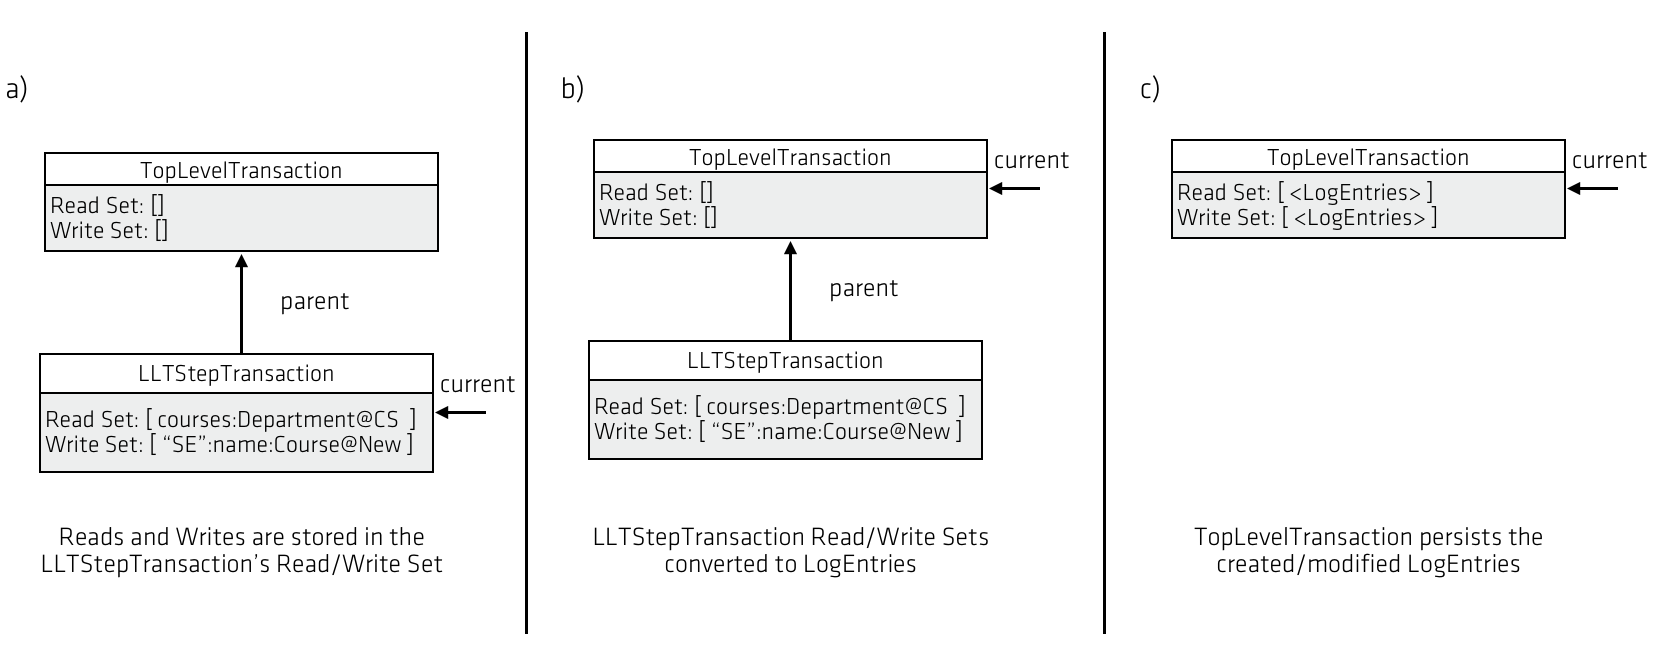
\includegraphics[width=1\linewidth]{llt-step-lifecycle}
\caption{LLTTransactionStep lifecycle}
\label{fig:llt-lifecycle}
\end{figure}

Figure~\ref{fig:llt-lifecycle} recaps the lifecycle of a
\texttt{LLTStepTransaction}. Figure \ref{fig:llt-lifecycle}a shows
that as the step is running, the {\it current} transaction is the
\texttt{LLTStepTransaction}, as such, reads and writes are kept in its
Read/Write Sets. During the commit of the step
(\ref{fig:llt-lifecycle}b), the {\it current} transaction is the
parent (backend-specific), and the \texttt{LLTStepTransaction}'s
Read/Write Sets are converted into \texttt{LogEntries}, written to the
parent's Write Set. Finally, once all the \texttt{LogEntries} are
created, the parent transaction is committed, persisting the step's
changes (\ref{fig:llt-lifecycle}c).

\subsubsection{Finishing the Long Lived Transaction}
\label{sec:jvstm-commit}

Once all steps of the Long Lived Transaction are finished, the LLT
must be committed, ensuring that the changes performed in it are
visible to the outside world. Much of this process is heavily
dependent on the backend as it involves direct access to the
underlying data structures.

The commit process of a Long Lived Transaction occurs within a regular
transaction. In this process, the data collected throughout the
multiple steps is validated and replayed. Once this transaction
commits, all written data will be merged with the global state of the
application.

The first step in committing the LLT is verifying whether all the read
data is still valid. As every slot is mapped in a JVSTM VBox, all the
boxes corresponding to the read slots must be verified. The process
iterates over all read slots, locating the VBox that represents the
slot. It then reads the VBox, so that it is added to the Read Set of
the current transaction. Then, the latest version of the VBox is
compared to context's version, thus ensuring that the read value was
the latest. If the box's current version if posterior to the read
version, the Long Lived Transaction is aborted.

There is a critical subtlety in this verification
process. Modifications to the VBox's underlying data structures are
performed only at commit time, inside a commit lock. As the
verification process is not run within the commit lock, it is possible
for another transaction to concurrently update a VBox after the
validation. Preventing incorrect behaviour is quite simple: Just read
the box. By doing this, the box will be validated when the transaction
commits, ensuring that the verification was correct (i.e. the version
read during the verification is still valid).

Consider the following scenario: VBox A was read in a Long Lived
Transaction in version 1 and not changed afterwards. When the Long
Lived Transaction commits (in a transaction X), A will be validated,
its current version (1) compared to the version of the transaction
(1). It passes the test and validation succeeds, proceeding with the
commit. Concurrently (after the validation, before X commits), another
transaction writes to A and commits, increasing its version to (X+1). When
X attempts to commit, its read set (which mirrors the Read Set of the
Long Lived Transaction) is validated. As A was concurrently written, X
will be restarted, and the version verification will fail, marking the
Long Lived Transaction as conflicting.

Once the Read Set of the Long Lived Transaction is validated, the
Write Set must be merged into the global state of the
application. This process iterates over the written slots, and for
each slot: (1) Locates the VBox representing it, (2) Converts the JSON
value to the concrete value, and (c) Writes the value to the VBox.

After the merge process is finished, the committing transaction has a
full mirror of the LLT's Read and Write Sets, and once it commits,
every change in the Write Set is available to the outside world.

\subsection{Validation}
\label{sec:validation}

This chapter proposed a solution that allows programmers to take
advantage of Long Lived Transactions with little effort and no code
modifications. I shall now validate the proposed solution, both in
terms of correctness and ease of use.

\subsubsection{Correctness}

One of the greatest challenges when implementing Long Lived Transactions
is ensuring that the solution provides the same correctness guarantees
as regular transactions. I will now demonstrate that the proposed
solution provides the same correctness guarantees as regular transactions.

Transactions in the JVSTM satisfy the Opacity correctness properties
(refer to Section~\ref{sec:opacity}). When integrated with the Fenix
Framework, transactions may also provide the Durability property,
depending on whether the concrete backend supports persistence.

The proposed solution also all the ACID properties for Long
Lived Transactions, as well as the Opacity correctness property.

\begin{itemize}

\item {\bf Atomicity} is provided as all the writes performed during
  the LLT are only written to the global state of the application when
  the it commits, which is performed by a regular transaction.

\item {\bf Consistency} is provided in the same way as a regular
  transaction, by ensuring that every read is still valid at commit
  time.

\item {\bf Isolation} is provided as no data is ever written to the
  global context until the LLT is finished, and data reads are isolated.

\item {\bf Durability} is provided if the underlying backend supports
  data persistence.

\end{itemize}

Throughout the execution of the Long Lived Transaction, written data
is collected and stored inside the \texttt{TransactionalContext}. Once
the transaction is finished, written data is {\bf atomically} written
to the global context, using a regular transaction which simply reads
data from one domain object (the context) to be written in another
(the actual objects written during the transaction).

Long Lived Transactions are {\bf consistent}. Similarly to regular
transactions, a LLT only commits if all the data read during the
transaction is still valid at commit time. This is done by comparing
the version of the LLT against the version of every box in the Read
Set, just like a regular transaction would do.

{\bf Isolation} is perhaps the hardest property to demonstrate. When
performing a read operation within a Long Lived Transaction, the
system ensures that the returned value will be the one at the moment
the first step of the LLT executed (i.e. the value consistent with the
transaction's version), just like it happens with regular
transactions.  As for writes, similarly to what happens with regular
transactions, written values are kept in transaction-local storage
(i.e. in \texttt{LogEntries}) and as such, can only be accessed by the
transaction itself.

{\bf Durability} is an ``optional'' property, as not all JVSTM-based
backends provide persistent support. Those that do however, ensure
that the effects of Long Lived Transactions are durable, as it works as
if writes occurred in a single regular transaction (which already
provides the Durability property).

I have shown that Long Lived Transactions provide the same correctness
guarantees as regular transactions. There is, however, one key piece
missing. Correctness is only guaranteed provided that all the
information about reads and writes is collected throughout the
transaction, and is available at commit time.

Recall from the previous sections that in each step of the Long Lived
Transaction, every read and write operation is intercepted, and for
each operation a record is created. Such records are kept in
\texttt{LogEntries}, which in turn are writting using regular
transactions. As such, once the LLT is committing, it is able to read
all the recorded data, and use it for all the necessary verifications
and data updates.

\subsubsection{Ease of Use}

The primary goal of this work is to ease the development of Long Lived
Transactions, and as such, it is rather important to provide a simple
and concise API.

The proposed solution fares well in that regard, as it allows existing
code to be adapted to use Long Lived Transactions with no
modifications. It is possible to program the business logic of your
whole application using regular transactions, and with a simple
wrapper add Long Lived Transaction support.

Consider a Web Application wishing to share with its users the
benefits of Long Lived Transactions, by allowing each individual user
to keep a series of Long Operations. Support for this feature could be
added at an infrastructural level, by providing the user with a UI to
manage his Operations (creating, committing, enabling, etc). Creating
and committing the operation would imply simple domain object
manipulation (in particular creating and committing a
\texttt{TransactionalContext}).

Making every action performed by the user as a step of the Long Lived
Transaction would be as simple as keeping the context in session-local
storage, and binding it before every transaction start (using a Web
Filter or similar). Listing~\ref{list:webFilter} shows a possible
implementation of a Web Filter to accomplish the desired behaviour.

With this architecture, it is possible to make every operation in the
application part of a Long Lived Transaction, without the need to
change existing code, or changing the methodology used to develop new
functionalities.

\begin{lstlisting}[caption={Web Filter to wrap every transaction in a
    TransactionalContext},label={list:webFilter},float]
public void doFilter(ServletRequest request, 
                     ServletResponse response, FilterChain chain) {
  HttpSession session = request.getSession();
  TransactionalContext ctx = session.getAttribute(LONG_TX_SESSION_PARAM);
  if (ctx == null) {
    chain.doFilter(request, response);
  } else {
    LongTransaction.setContextForThread(ctx);
    try {
      chain.doFilter(request, response);
    } finally {
      LongTransaction.removeContextFromThread();
    }
  }
}
\end{lstlisting}

%% Optimization

\section{Optimization}

The solution presented in Section~\ref{chap:solution}, despite
providing correctness guarantees and ease of use, performs poorly even
in trivial test cases. This chapter describes a series of
optimizations made to keep the overhead as low as possible, without
sacrificing correctness.

\subsection{Example Application}

To perform accurate measurements, I developed a sample banking
application. In this application's domain there is a central Bank with
Customers, which in turn have their accounts. For each account the
application keeps its balance, and there is a method to show a
customer's balance (by summing the balance of all his accounts). Every
time a banking transaction (transfer, deposit, etc.) is done, a new
\texttt{TransactionRecord} is created, containing a timestamp, the
origin and destination accounts, as well as the amount transfered.

In this scenario, a Business Transaction will consist of several
banking transactions, spread throughout a series of Business
Operations. This is the perfect candidate for a Long Lived
Transaction.

Using this banking domain, a sample application was developed. In this
fictitious scenario, the bank starts with a certain number of
customers (this number is configurable so that different parameters
may be measured) and a configurable number of operations. Within each
operation, new customers and accounts are created, money is shuffled
between all the accounts of every customer (creating a new
TransactionRecord for each transaction), and the total balance is
calculated. This means that in each step: (1) every object in the
system is read, (2) many objects are written and (3) many new objects
are created.

In the {\it regular} scenario, each business operation will run within
a regular JVSTM transaction (and thus every intermediate state is
visible to the outside world), whereas in the {\it Long Lived}
scenario the Business Transaction is mapped into a Long Lived
Transaction, and each individual operation runs within an LLT step
(meaning that intermediate state will not be visible to the outside).

With the support presented in previous sections, the programmer simply
writes the application's code as he would without considering Long
Lived Transactions. No changes to the data structures and business
logic are required. Listing~\ref{lst:invoc-diff} shows the two methods
used to invoke both versions under test. Notice that they both look
very similar as they both invoke the \texttt{doScript} method, the
only difference is that in the LLT version, a new
\texttt{TransactionalContext} is created and bound to the current
thread.

\begin{lstlisting}[caption={Invoking the business operation},
 label={lst:invoc-diff},float]
public void doRegular() {
  doScript("regular");
}

public void doLongTx() {
  TransactionalContext context = createContext();
  LongTransaction.setContextForThread(context);
  doScript("long");
  LongTransaction.removeContextFromThread();
}

public void doScript(String scriptName) {
  for(int i = 0; i < NUMBER_OF_OPERATIONS; i++) {
    doOperation();
  }
}
\end{lstlisting}

\subsection{Initial Performance Analysis}

Figure~\ref{fig:regTime} shows the running time for a varying number
of operations of the application presented above. As expected, the
running time grows linearly as the number of operations increases.

When looking at the Long Lived version (where every operation is a
step of one large Long Lived Transaction), performance quickly
degrades as the number of operations grows. The main reason for this
performance hit is that every box read will cause many other boxes to
be read (instead of just reading the box directly, all LogEntries
representing the write set must be traversed, meaning that many more
boxes are read along the way, and many more boxes will be read as the
transaction grows in size). Recall from Section~\ref{chap:ff} that in
the JVSTM using a multi-box layout, each slot of an object is kept in
a separate box, and as such reading a single Log Entry will cause at
least 3 boxes to be read: the slot name, the target object, and the
next box in the list.

As reading boxes is one of the major sources of the poor performance
results of this implementation, I made several improvements regarding
the number of boxes read and boxes written. The next sections present
those optimizations.

\begin{figure}
\centering
\begin{minipage}{.5\textwidth}
  \centering
  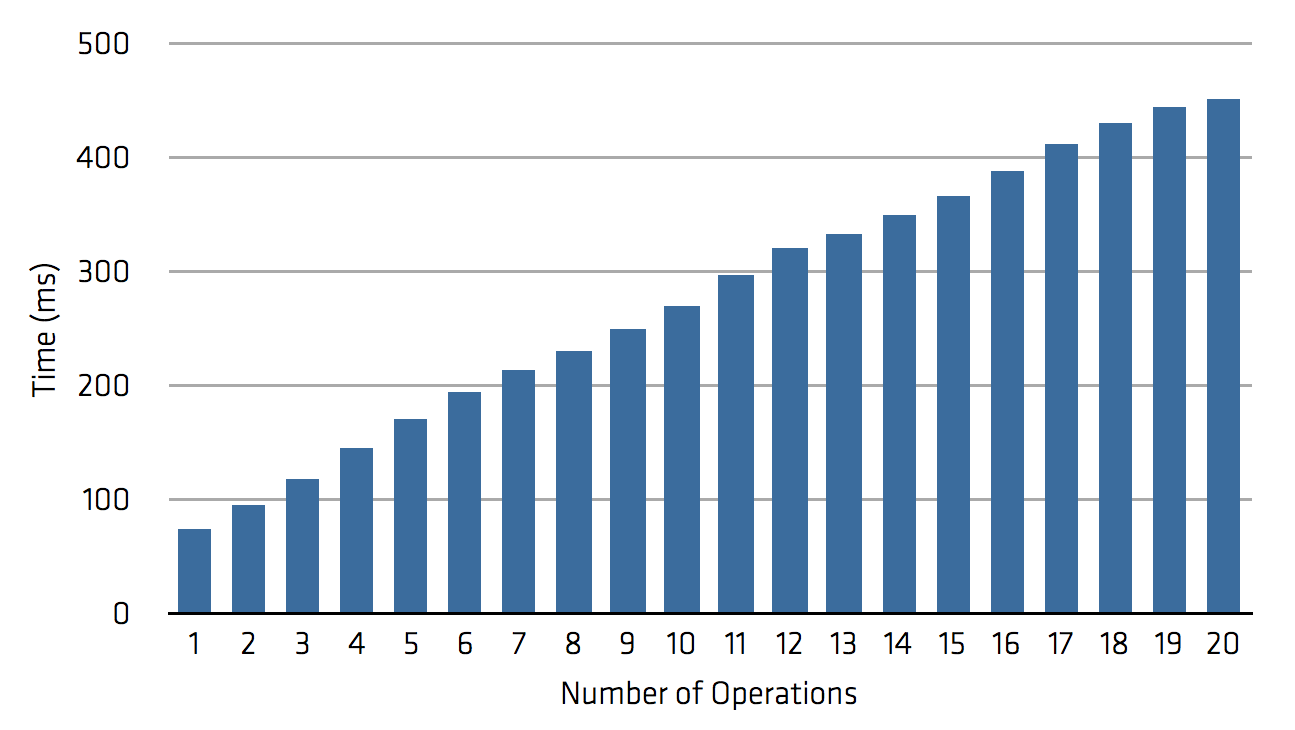
\includegraphics[width=1\linewidth]{time-regular}
  \caption{Running time with regular transactions}
  \label{fig:regTime}
\end{minipage}%
\begin{minipage}{.5\textwidth}
  \centering
  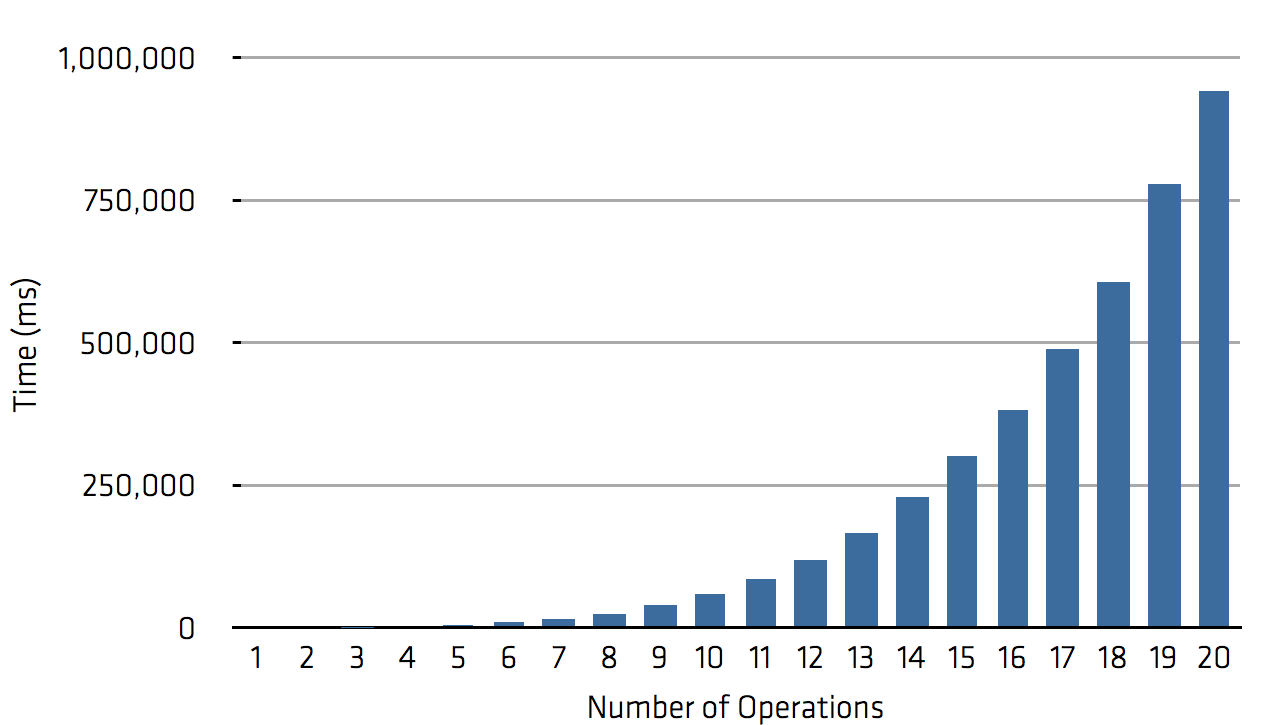
\includegraphics[width=1\linewidth]{time-long-v1}
  \caption{Running time with Long Lived Transaction steps}
\end{minipage}
\end{figure}

\subsection{Read-Set differentiation}

In the initial implementation, \texttt{LogEntries} were used to reify
both the Read Set and the Write Set.

Recalling Figure \ref{fig:transactionalContext}, \texttt{LogEntries}
store a reference to the DomainObject they refer to, the name of the
slot, and the slot's value. Using the same objects to represent both
sets proved to be quite expensive, as the Read Set only cares about
which slots were read, completely ignoring its value.

By analysing the nature of the Read Set, we may conclude that it is
only necessary to store the pairs [DomainObject, Slot] read by the
transaction (the actual version read is not relevant, as it will
always be coherent with the transaction's version).

As such, the Read Set has been replaced by an immutable
ValueType,\footnote{ValueTypes are explained in detail in Section
  \ref{chap:ff}.} containing a set of DomainSlotKey's (an immutable,
lightweight object representing the pair [DomainObject, Slot]), stored
directly into the \texttt{TransactionalContext}.

This optimization greatly reduced the space required by the
Transaction (both in-memory and persistently), as the representation
of the Read-Set became more compact (a single slot in an object vs
several objects).

The commit time for the various steps of the Transaction also
improved, as the lookups/insertions of entries in the Read Set are
done entirely in memory, without the need to traverse (and
potentially reload a large object graph).

\subsection{Using BPlusTrees to hold LogEntries}

As described in Section \ref{chap:ff}, the Fenix Framework uses
BPlusTrees and other collections to implement to-many relations. These
collections are transparently handled by the Framework, and are
implemented using regular Domain Objects (such as Leaf Nodes and Inner
Nodes). As keeping track of changes in relations is a requirement for
our implementation, it is critical that changes to BPlusTrees are
correctly tracked.

This posed a great issue, as conceptually one
\texttt{TransactionalContext} has many \texttt{LogEntries} in both its
Read and Write Sets. If theses relations were to be implemented using
regular one-to-many relations, a BPlusTree would be generated by the
Framework. But as BPlusTrees must be tracked by the
\texttt{TransactionalContext}, they could not be used to implement
this relation.

The initial approach to this problem consisted on implementing the
relation using a Linked List, in which a LogEntry would be directly
connected to the next one in the list, keeping the list sorted by
insertion order. This approach proved to be quite inefficient, as
lookups in the Write Set were {\it O(n)} in the number of written
objects, making it impractical, as every \texttt{getBoxValue}
operation required potentially traversing the whole list.

To solve this issue, a specialised \texttt{WriteSetBPlusTree} was
developed. The major difference between a \texttt{WriteSetBPlusTree}
and a regular BPlusTree is that the former is designed to be kept out
of the scope of the TransactionalContext, making it possible to use it
to implement the one-to-many relation between a TransactionalContext
and its LogEntries.

Another advantage of directly using a BPlusTree is that it is possible
to take full advantage of all its features. Generically speaking, a
BPlusTree is a map between keys and values. When the Fenix Framework
generates a BPlusTree to represent a to-many relation, the map
contains the pointed objects as values, and the object's identifiers
(OID) as keys. In this case however, lookups are not performed by OID,
but by DomainSlotKey (DomainObject+slot). As such, a WriteSetBPlusTree
will map DomainSlotKeys to their corresponding LogEntries.

With this approach, looking up a DomainSlotKey in a
TransactionalContext means that the BPlusTree is indexed using the
DomainSlotKey, and as such, lookup times are now {\it O(log(n))}.

In Figure~\ref{fig:comparisonBPlus} we can
see that the running time using BPlusTrees is closer to the regular
version. However, the growth rate (while linear) is still bigger than
the original, with the benchmark taking on average 4.4x to
complete. One of the big contributors for this speed improvement seems
to be the number of Box Reads that happens throughout the
transaction. Whereas in the original implementation this number
reached over 8.7B, it is now reduced to about 2.1M.



\subsection{Removing LogEntries}

With the relation between the \texttt{TransactionalContext} and the
\texttt{LogEntries} implemented using a BPlusTree, another issue
arisen.

Despite having great lookup times, the commit of a Long Transactions's
step was greatly affected. Whereas inserting elements in a Linked List
is {\it O(1)}, the insertion in the BPlusTree was still painfully
slow.

This is because the Fenix Framework requires that ValueTypes (such as
the ones used to back the BPlusTree) are immutable combined with the
fact that the BPlusTree provides no API for batch insertion, meaning
that for each of the elements written within a given step, a new
insert was performed, and the backing TreeMaps were duplicated over
and over. 

The approach to solve this issue, was to use a solution similar to the
one used for the Read-Set: create an immutable ValueType, containing
the mapping between all written slots and their respective values.

With this change, \texttt{LogEntries} were completely taken out of the
picture, as the only extra piece of information they provided was the
JSON contents of the slot, which could be embedded directly into the
WriteSet object.

The issue with this approach is that, due to the immutability
requirement, every time a batch of entries was inserted, the whole Map
had to be duplicated, which was rather wasteful both in terms of time
and allocated memory. So, instead of duplicating the whole Map, the
WriteSet is actually a Linked-List of Maps, containing one node per
transaction step. This means that the performance of lookups is now
{\it O(s*log(n))}, {\it n} being the average size of each step, and
{\it s} the number of steps (in which something is written) of the
transaction.

There is, however, a tradeoff. Transactions with a small number of large
steps (which is the typical use case) are greatly improved (as lookups
in an in-memory hash map are fast), however transactions with a large
number of small steps take a major performance hit, as a new node is
created in every step with small amounts of information.

As such, a new node is only created if the current node has size above
a certain (user-defined) threshold. This threshold defines whether it
is more cost-effective to create a new node (which is practically
instant on insertion but makes lookups more expensive) or replace the
current one (thus duplicating the map). The user can set the threshold
to be lower or higher according to the usage patterns of the
application.

Applications with a large number of small steps benefit from a large
threshold, as insertions will be quite cheap and have little to no
impact on lookups. On the other hand, applications with a small number
of large steps should set the threshold lower than the average size of
a step, so that there is no need to duplicate a potentially large map.

\subsection{Final Performance Analysis}

After applying all the optimizations described throughout this
chapter, the solution provides quite competitive
results. Figure~\ref{fig:comparisonFinal} shows a runtime comparison
between using regular transactions and the final implementation of
Long Lived Transactions: The slow down is now under 40\%.

The number of Box Reads is also very close to the regular transaction
version, adding very little overhead. As the Write and Read Sets are
now represented in specialised data structures, it is no longer
necessary to read vast amounts of VBoxes just to determine whether a
given element is in one of the sets. 

There is also one very important measurement that has not been
mentioned thus far: The performance impact of the solution in regular
transactions. A solution in which Long Lived Transactions are
performant at the cost of having expensive regular transactions is not
an acceptable one. For the proposed solution, there is close to zero
overhead on starting regular transactions. The only performance hit is
the added verification upon starting a new transaction, to check
whether the current thread if bound to a
\texttt{TransactionalContext}. Other than that, no changes were made
that would affect the performance of regular transactions.

\begin{figure}
\centering
\begin{minipage}{.5\textwidth}
  \centering
  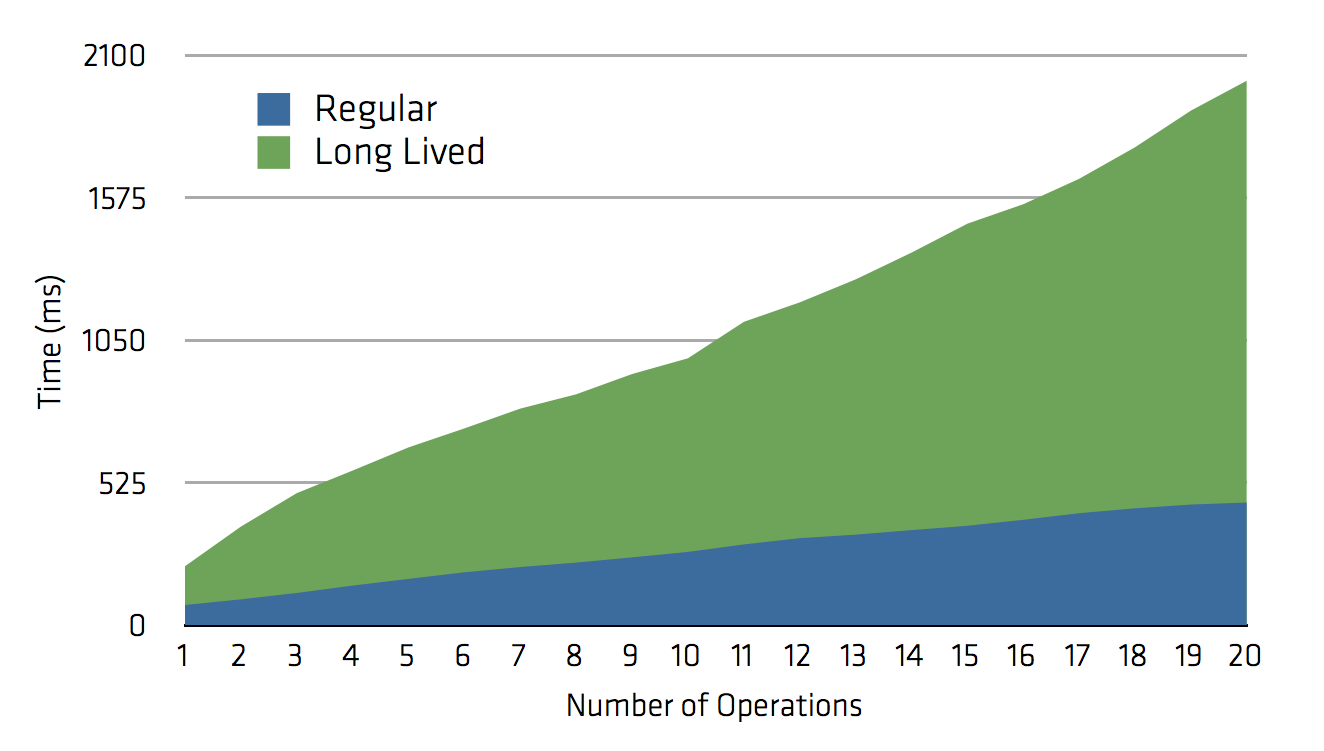
\includegraphics[width=0.9\linewidth]{comparison-bplus}
  \caption{Running time comparison using BPlusTrees}
  \label{fig:comparisonBPlus}
\end{minipage}%
\begin{minipage}{.5\textwidth}
  \centering
  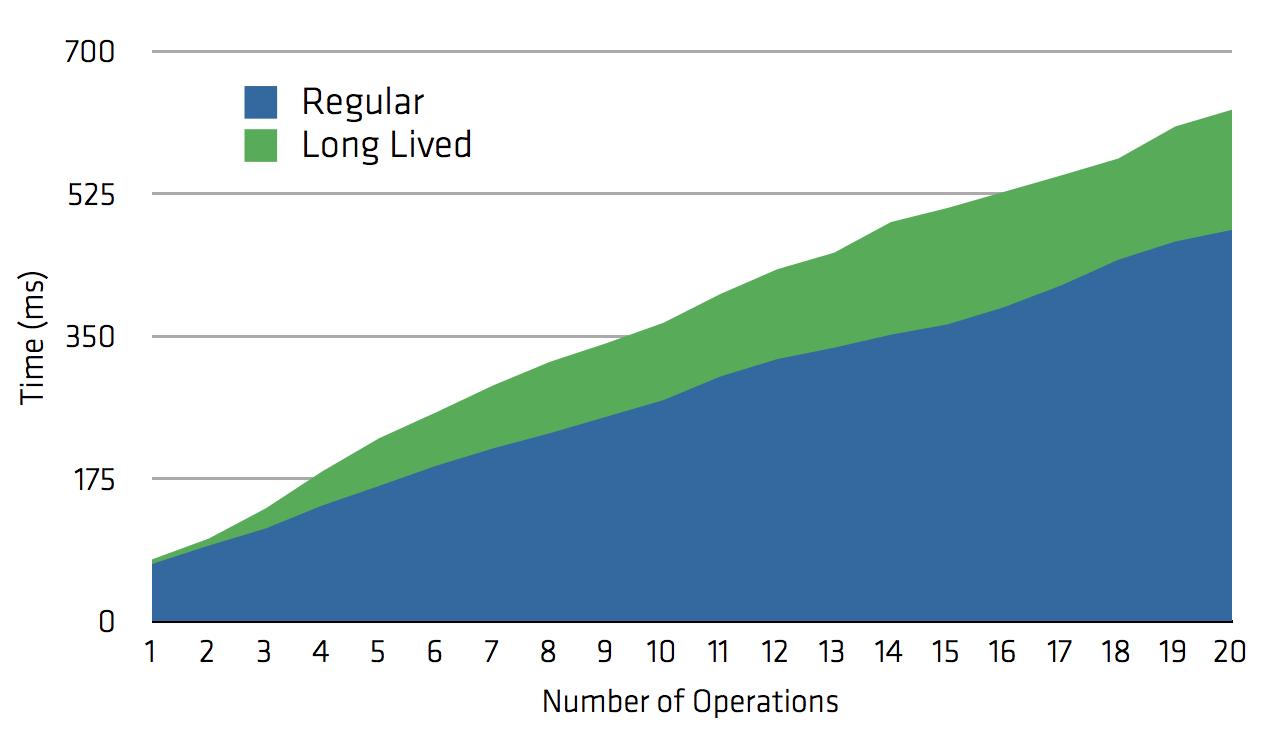
\includegraphics[width=0.9\linewidth]{comparison-final}
  \caption{Running time comparison for the Final Implementation}
  \label{fig:comparisonFinal}
\end{minipage}
\end{figure}

%% Conclusion

\section{Conclusion}

Many enterprise applications have requirements involving operations
that may span arbitrarily long periods of time. Yet, most modern data
persistence frameworks are lackluster in regard to Long Lived
Transactions. This forces programmers to devise clever ways to
implement their requirements, promoting bad engineering practices and
adding unnecessary complexity to the system.

The Fenix Framework, as a Framework to support enterprise applications
that require a persistent and transactional rich domain model, merely
provided support for regular (short-lived) transactions, and as such,
suffered from the same perils of many other frameworks.

This document has described an extension to the Fenix Framework that
allows drop-in support for Long Lived Transactions, without the need
to modify existing business code. The presented extension shows
many characteristics desirable of such a solution. These include
support for system restarts by storing intermediate data persistently,
support for concurrent users collaborating on a single Long Lived
Transaction, the same correctness guarantees as regular transactions
as well as comparable performance on the execution of the
transaction's steps.

The initial implementation, while fully functional, present very poor
performance results, rendering even the simplest of test cases
unusable. I then presented an in-depth analysis of the implementation,
and was able to track down the reasons for such poor performance. By
doing several improvements on how the intermediate data is stored and
search, I was able to accomplish very good performance results,
providing execution times close to those of regular transactions.

~\\

Overall I believe that this work was rather successful, I was able to
develop a solution that allows programmers to take advantage of Long
Lived Transactions with minimal modifications to existing code, which
was the primary goal of this dissertation.

\bibliography{biblio.bib} \bibliographystyle{plain}
\end{document}